\chapter{Specifikacija programske potpore}
		
	\section{Funkcionalni zahtjevi}
			
			\textbf{\textit{dio 1. revizije}}\\
			
			
			\noindent \textbf{Dionici:}
			
			\begin{packed_enum}
				
				\item Znanstvena udruga "Pametna ekipa" (naručitelj)
				\item Registrirani korisnici (korisnici koji se mogu prijaviti u sustav)
				\begin{packed_enum}
					\item Sudionik
					\item Recenzent
					\item Predsjedavajući konferencije				
					\item Administrator
				\end{packed_enum}
				\item Razvojni tim
				
			\end{packed_enum}
			
			\noindent \textbf{Aktori i njihovi funkcionalni zahtjevi:}
			
			
			\begin{packed_enum}
					\item  \underbar{ Neregistrirani/neprijavljeni korisnik (inicijator) može:}
				
				\begin{packed_enum}
					
					\item pristupiti naslovnici konferencije i sadržaju na njoj, kao i stranici s informacijama o samoj konferenciji
					\item registrirati se - stvoriti novi korisnički račun za koji su mu potrebni osobni podaci - ime i prezime, naziv matične ustanove (kao i ulica i kućni broj, grad i država institucije), e-mail adresa; korisnik koji se registrira kao sudionik konferencije unosi i naslov rada, autore te e-mail adresu autora koji je osoba za kontakt 
					\item prijaviti se u sustav (ukoliko se prethodno registrirao)
					\item na stranici prijave zatražiti novu lozinku (ukoliko se prethodno registrirao)
					
				\end{packed_enum}
			 	\item  \underbar{Registrirani korisnik (inicijator):}
			 
			 	\begin{packed_enum}
					\item  \underbar{Sudionik (inicijator) može:}
				
					\begin{packed_enum}
					
						\item pregledavati i mijenjati osobne podatke 
						\item učitati rad u \textit{.pdf} formatu (do kraja roka za predaju)
						\item po potrebi priložiti izmijenjenu verziju rada i pri tome obavijestiti recenzenta u učinjenome
						\item ako želi predati dodatni rad 
					
					
					\end{packed_enum}
				
					\item  \underbar{Recenzent (inicijator) može:}
				
					\begin{packed_enum}
					
						\item pregledavati i mijenjati osobne podatke 
						\item pregledavati pristigle radove
						\item preuzeti radove na lokalno računalo
						\item prihvatiti rad bez izmjena
						\item prihvatiti rad uz manje izmjene, bez naknadnih provjera
						\item odobriti rad uz veće izmjene, pri čemu mora obavijestiti autora te ponovno pregledati izmijenjeni rad
						\item u potpunosti odbiti rad, pri čemu je potrebno navesti razloge i objasniti ocjenu
					
					
					\end{packed_enum}
				
					\item  \underbar{Predsjedavajući konferencije (inicijator) može:}
				
					\begin{packed_enum}
						
						\item pregledavati i mijenjati osobne podatke 
						\item vidjeti sve podatke o sudionicima, mijenjati ih i dodavati sadržaj
						\item preuzeti sve pristigle radove na lokalno računalo
						\item dati odobrenje za obavljanje recenzije radova recenzentima
						\item svima ili samo odabranim korisnicima slati obavijesti na e-mail
					
				
					\end{packed_enum}
				
					\item  \underbar{Administrator (inicijator) može:}
				
					\begin{packed_enum}
						
						\item pregledavati i mijenjati osobne podatke 
						\item upisati podatke o konferenciji
						\item odrediti predsjedavajućeg konferencije
						\item pratiti stanje COVID-19 pandemije putem javno dostupnih podataka o incidenciji u državama iz kojih ima prijavljenih sudionika
						\item učiniti radove javno dostupnima u slučaju pogoršanja epidemiološke situacije
						\item definirati upitnik za prijavu na konferenciju
						\item vidjeti broj i imena aktivno registriranih korisnika
						\item pregledavati statistiku (broj radova) prijava po državama, sekcijama
						\item pregledavati i mijenjati podatke sudionika
						\item poslati obavijest pojedinim ili svim sudionicima 

					\end{packed_enum}
				\end{packed_enum}


				\item \underbar{Baza podataka (sudionik):}

				\begin{packed_enum}

					\item pohranjuje podatke o korisnicima i njihovim ovlastima u sustavu
					\item pohranjuje podatke o radovima, njihovim autorima i recenzijama tih radova
					\item pohranjuje podatke o konferenciji i upitniku za prijavu na konferenciju
					\item pohranjuje podatke o ustanovama iz kojih dolaze registrirani sudionici

				\end{packed_enum}
					
			\end{packed_enum}
			
			\eject 
			
			
				
			\subsection{Obrasci uporabe}
				
				\textbf{\textit{dio 1. revizije}}
				
				\subsubsection{Opis obrazaca uporabe}
					
					\noindent \underbar{\textbf{UC1 - Pregled naslovnice}}
					\begin{packed_item}
	
						\item \textbf{Glavni sudionik: } Neregistrirani korisnik, registrirani korisnik
						\item  \textbf{Cilj:} Pregledavanje statičnog sadržaja stranice
						\item  \textbf{Sudionici:} Baza podataka
						\item  \textbf{Preduvjet:} -
						\item  \textbf{Opis osnovnog tijeka:}
						
						\item[] \begin{packed_enum}
	
							\item Otvaranjem linka na stranici se prikazuje statičan sadržaj
							\item Pregledavanje sadržaja
						\end{packed_enum}
						

					\end{packed_item}

					\noindent \underbar{\textbf{UC2 - Registracija}}
					\begin{packed_item}
	
						\item \textbf{Glavni sudionik: } Neregistrirani korisnik
						\item  \textbf{Cilj:} Stvaranje novog korisničkog računa za pristup aplikaciji
						\item  \textbf{Sudionici:} Baza podataka
						\item  \textbf{Preduvjet:} Korisnik nema račun
						\item  \textbf{Opis osnovnog tijeka:}
						
						\item[] \begin{packed_enum}
	
							\item Korisnik odabire opciju "Registracija" nakon čega se otvara obrazac za registraciju
							\item Korisnik ispunjava obrazac
							\item Korisnik odabire kreira li račun kao sudionik ili recenzent, te ukoliko odabere opciju sudionik pojavljuje se još jedan dio obrasca gdje je potrebno unijeti naziv rada koji želi predati i autore istog te označiti osobu za kontakt
							\item Sustav svakom sudioniku pridjeljuje jedinstveni identifikator ID\_xxxx, pri čemu je xxxx redni broj prijave u sustav
							\item Ažurira se baza podataka
							\item Korisnik koji se registrirao kao sudionik konferencije prima obavijest (putem e-maila) o uspješnoj registraciji (koju je potrebno potvrditi "klikom" na dobiveni link) u kojoj se nalazi lozinka za prijavu, a recenzent tu obavijest prima po odobrenju predsjedavajućeg
							
						\end{packed_enum}

						\item  \textbf{Opis mogućih odstupanja:}
						
						\item[] \begin{packed_item}
	
							\item[2.a]  Odabir već zauzetog e-maila, unos jednog ili više korisničkih podataka u nedozvoljenom formatu, postoji već rad s tim naslovom i istim autorima
							\item[] \begin{packed_enum}
								
								\item Sustav korisniku daje obavijest o tome gdje je nastala greška pri registraciji
								\item Korisnik sukladno mijenja unesene podatke sve dok nisu svi potrebni podaci ispravno upisani, odnosno u odgovarajućem formatu
								
							\end{packed_enum}
							\item[2.b]  Korisnik nije ispunio neko polje obrasca koje je označeno kao obavezno
							\item[] \begin{packed_enum}
								
								\item Sustav korisniku daje obavijest o tome koje polje nije ispunjeno i da ga mora ispuniti.
								
							\end{packed_enum}
							
						\end{packed_item}
			
					\end{packed_item}

					\noindent \underbar{\textbf{UC3 - Prijava u sustav}}
					\begin{packed_item}
	
						\item \textbf{Glavni sudionik: } Registrirani korisnik
						\item  \textbf{Cilj:} Dobiti pristup korisničkom sučelju
						\item  \textbf{Sudionici:} Baza podataka
						\item  \textbf{Preduvjet:} Odrađena uspješna registracija
						\item  \textbf{Opis osnovnog tijeka:}
						
						\item[] \begin{packed_enum}

							\item Korisnik na naslovnici ili u glavnog izborniku bira opciju "Prijava", nakon čega se učitava stranica za prijavu
							\item Unos korisničkog e-maila i lozinke
							\item Korisnik može kliknuti gumb "Zaboravljena lozinka" te mu se generira nova (UC 3.1)
							\item Potvrda o ispravnosti unesenih podataka
							\item Pristup korisničkom sučelju
					
						\end{packed_enum}

						\item  \textbf{Opis mogućih odstupanja:}
						
						\item[] \begin{packed_item}
	
							\item[2.a]  Neispravan e-mail ili lozinka
							\item[] \begin{packed_enum}
								
								\item Sustav korisniku daje obavijest o neispravno unesenim podacima, omogućuje novi unos podataka za prijavu te upućuje korisnika da ukoliko nije izvršena registracija prvo napravi taj korak
								
							\end{packed_enum}
							
						\end{packed_item}
			
					\end{packed_item}
				\noindent \underbar{\textbf{UC3.1 - Zahtjev za dobivanje nove lozinke}}
				\begin{packed_item}
					
					\item \textbf{Glavni sudionik: } Registrirani korisnik
					\item  \textbf{Cilj:} Dobiti novu lozinku
					\item  \textbf{Sudionici:} Baza podataka
					\item  \textbf{Preduvjet:} Korisnik je registriran, ali nije prijavljen u sustav
					\item  \textbf{Opis osnovnog tijeka:}
					
					\item[] \begin{packed_enum}
				
						\item Korisniku je učitana stranica za prijavu te je on kliknuo na gumb "Zaboravljena lozinka"
						\item Od korisnika se traži da unese e-mail na koju će mu biti poslana nova lozinka
						\item Generira se lozinka i šalje korisniku
						\item Aplikacija obavještava korisnika da mu je lozinka poslana na e-mail
						\item Ažurira se baza podataka
						
					\end{packed_enum}
					
					\item  \textbf{Opis mogućih odstupanja:}
					
					\item[] \begin{packed_item}
						
						\item[2.a]  Neispravan format e-maila i/ili e-mail ne postoji u bazi podataka
						\item[] \begin{packed_enum}
							
							\item Sustav korisniku daje obavijest o neispravno unesenim podacima, ponovno učitava stranicu za prijavu te upućuje korisnika da ukoliko nije izvršena registracija prvo napravi taj korak
							
						\end{packed_enum}
						
					\end{packed_item}
					
				\end{packed_item}
					\noindent \underbar{\textbf{UC4 - Pregled osobnih podataka}}
					\begin{packed_item}
						
						\item \textbf{Glavni sudionik: } Registrirani korisnik
						\item  \textbf{Cilj:} Pregledati osobne podatke
						\item  \textbf{Sudionici:} Baza podataka
						\item  \textbf{Preduvjet:} Korisnik je prijavljen u sustav
						\item  \textbf{Opis osnovnog tijeka:}
						
						\item[] \begin{packed_enum}
							
							\item Korisnik klikom na gumb "Moj profil" otvara stranicu svog profila
							\item Aplikacija prikazuje osobne podatke o korisniku povučene iz baze podataka
							\item Korisnik ima mogućnost promjene osobnih podataka (UC4.1)
							
						\end{packed_enum}
						
					\end{packed_item}
					\noindent \underbar{\textbf{UC4.1 - Promjena osobnih podataka}}
					\begin{packed_item}
						
						\item \textbf{Glavni sudionik: } Registrirani korisnik
						\item  \textbf{Cilj:} Izmijeniti osobne podatke
						\item  \textbf{Sudionici:} Baza podataka
						\item  \textbf{Preduvjet:} Korisnik je prijavljen u sustav
						Korisnik ima otvorenu stranicu svog profila
						\item  \textbf{Opis osnovnog tijeka:}
						
						\item[] \begin{packed_enum}
							
							\item Korisnik odabere opciju "Promijeniti" kraj osobnih podataka
							\item Korisnik radi željene izmjene
							\item Korisnik odabire opciju "Spremi promjene"
							\item Baza podataka se ažurira
							
						\end{packed_enum}
						
						\item  \textbf{Opis mogućih odstupanja:}
						
						\item[] \begin{packed_item}
							
							\item[3.a]  Korisnik izvrši promjenu podataka, ali uneseni podaci nisu u ispravnom formatu
							\item[] \begin{packed_enum}
								
								\item Sustav ne dozvoljava spremanje izmjena dok podaci nisu u ispravnom formatu
								\item Sustav kraj podatka koji je neispravno zapisan prikaže obavijest kako podatak nije u ispravnom formatu te upućuje da korisnik ispravi isto
								
							\end{packed_enum}
							
							\item[3.b]  Korisnik izvrši promjenu podataka, ali ne odabere opciju "Spremi promjene"
							\item[] \begin{packed_enum}
								
								\item Sustav obavještava korisnika da nije spremio podatke prije izlaska iz prozora
								
							\end{packed_enum}
							
						\end{packed_item}
						
					\end{packed_item}

				
					\noindent \underbar{\textbf{UC5 - Predaja rada}}
					\begin{packed_item}
	
						\item \textbf{Glavni sudionik: } Sudionik konferencije
						\item  \textbf{Cilj:} Predati rad koji je prijavio pri registraciji
						\item  \textbf{Sudionici:} Baza podataka
						\item  \textbf{Preduvjet:} Korisnik je prijavljen u sustav, prvi rad još nije predan (.pdf nije učitan i pohranjen)
						\item  \textbf{Opis osnovnog tijeka:}
						
						\item[] \begin{packed_enum}

							\item Korisnik bira gumb "Moji radovi" iz glavnog izbornika
							\item Na stranici "Moji radovi" korisnik odabire opciju "Predaj rad" kraj željenog rada
							\item Pojavljuju se već ispunjena polja s nazivom rada i skupom autora koje je korisnik pri registraciji naveo, korisnik odabire opciju "Učitaj rad".
							\item Korisnik učitava rad u .pdf formatu
							\item Korisnik odabire opciju "Predaj"
							\item Rad se pohranjuje i baza podataka se ažurira
							\item Sustav šalje obavijest korisniku o uspješno predanom radu

					
						\end{packed_enum}

						\item  \textbf{Opis mogućih odstupanja:}
						
						\item[] \begin{packed_item}
	
							\item[4.a]  Korisnik je učitao datoteku koja nije u *.pdf obliku
							\item[] \begin{packed_enum}
								
								\item Sustav javlja da je dozvoljeno učitavati isključivo .pdf dokumente i ne pohranjuje ono što je korisnik pokušao prenijeti
								
							\end{packed_enum}

							\item[5.a]  Korisnik prenese datoteku, ali ne odabere opciju "Predaj"
							\item[] \begin{packed_enum}
								
								\item Sustav javlja korisniku kako nije pohranio rad prije izlaska iz prozora
								
							\end{packed_enum}
							
						\end{packed_item}
					
					\end{packed_item}
					
					\noindent \underbar{\textbf{UC6 - Pregled vlastitih radova}}
					\begin{packed_item}
						
						\item \textbf{Glavni sudionik: } Sudionik konferencije
						\item  \textbf{Cilj:} Pregledati vlastite radove
						\item  \textbf{Sudionici:} Baza podataka
						\item  \textbf{Preduvjet:} Korisnik je prijavljen u sustav
						\item  \textbf{Opis osnovnog tijeka:}
						
						\item[] \begin{packed_enum}
							
							\item Korisnik klikne na gumb "Moji radovi" iz glavnog izbornika
							\item Aplikacija prikazuje popis predanih radova povučen iz baze podataka
							\item Korisnik odabire željeni rad s popisa te mu se otvara stranica s podatcima o radu
					
						\end{packed_enum}                
						
					\end{packed_item}
						\noindent \underbar{\textbf{UC7 - Predaja dodatnog rada}}
					\begin{packed_item}
						
						\item \textbf{Glavni sudionik: } Sudionik konferencije
						\item  \textbf{Cilj:} Predaja dodatnog rada
						\item  \textbf{Sudionici:} Baza podataka
						\item  \textbf{Preduvjet:} Korisnik je prijavljen u sustav, prethodno je predao minimalno jedan rad
						\item  \textbf{Opis osnovnog tijeka:}
						                                                                          
						\item[] \begin{packed_enum}
							\item Korisnik klikne na gumb "Moji radovi" iz glavnog izbornika
							\item Aplikacija prikazuje popis predanih radova povučen iz baze podataka
							\item Korisnik odabire opciju "Želim predati još jedan rad"
							\item Korisnik ispunjava formu za predaju dodatnog rada (autori, naziv, .pdf)
							\item Korisnik odabire opciju "Predaj rad"
							\item Korisniku se ponovno učitava stranica "Moji radovi" na kojoj je sada vidljiv novi rad
							\item Sustav šalje obavijest korisniku o uspješno predanom radu 
							
							
						\end{packed_enum}
						
						\item  \textbf{Opis mogućih odstupanja:}
						        
						\item[] \begin{packed_item}
							
							\item[4.a]  Korisnik je učitao datoteku koja nije u *.pdf obliku
							\item[] \begin{packed_enum}
								
								\item Sustav javlja da je dozvoljeno učitavati isključivo .pdf dokumente i ne pohranjuje ono što je korisnik pokušao prenijeti
								      
							\end{packed_enum}
							
							\item[5.a]  Korisnik prenese datoteku, ali ne odabere opciju "Predaj rad"
							\item[] \begin{packed_enum}
								
								\item Sustav javlja korisniku kako nije pohranio rad prije izlaska iz prozora
								
							\end{packed_enum}
							
						\end{packed_item}               
						
					\end{packed_item}
					
					\noindent \underbar{\textbf{UC8 - Izmjena rada po zahtjevu recenzenta}}
					\begin{packed_item}
						\item \textbf{Glavni sudionik:} Sudionik
						\item \textbf{Cilj:} Izmijeniti ranije učitan rad
						\item \textbf{Sudionici:} Baza podataka
						\item \textbf{Preduvjet:} Korisnik je prijavljen u sustav, recenzent dao ocjenu za koju je rad potrebno izmijeniti
						
						\item \textbf{Opis osnovnog tijeka:} 
						\item[] \begin{packed_enum}
							
							
							\item Korisnik klikne na gumb "Moji radovi" iz glavnog izbornika
							\item Aplikacija prikazuje popis predanih radova povučen iz baze podataka
							\item Korisnik odabire rad s popisa 
							\item  Korisniku se prikazuju podatci o radu odabranom s popisa vlastitih radova
							\item Korisnik učitava izmijenjeni rad u .pdf formatu
							\item Korisnik odabire opciju "Zaključaj predaju"
							\item Ako je rad ocijenjen da su potrebne veće izmjene, automatski se šalje e-mail recenzentu rada o obavljenoj izmjeni
							\item Rad se pohranjuje i baza podataka se ažurira
						\end{packed_enum}
						
						\item \textbf{Opis mogućih odstupanja:}
						\item[] \begin{packed_enum}
							\item[5.a] Korisnik je učitao datoteku koja nije u .pdf formatu
							\item[] \begin{packed_enum}
								\item[1.] Sustav javlja da je dozvoljeno učitati isključivo .pdf dokumente i ne pohranjuje ono što je korisnik pokušao prenijeti
							\end{packed_enum}
							
							\item[6.a] Korisnik prenese datoteku, ali ne odabere opciju "Zaključaj predaju"
							\item[] \begin{packed_enum}
								\item[1.] Sustav javlja korisniku kako nije pohranio rad prije izlaska iz prozora
							\end{packed_enum}
							
						\end{packed_enum}
					\end{packed_item}
					
					

				
					\noindent \underbar{\textbf{UC9 - Pregled recenzenata koji čekaju na odobrenje}}
					\begin{packed_item}
						
						\item \textbf{Glavni sudionik: } Predsjedavajući konferencije
						\item  \textbf{Cilj:} Odobriti registraciju recenzenta i poslati mu podatke za prijavu
						\item  \textbf{Sudionici:} Baza podataka
						\item  \textbf{Preduvjet:} Korisnik je prijavljen u sustav
						\item  \textbf{Opis osnovnog tijeka:}
						
						\item[] \begin{packed_enum}
							
							\item Korisnik odabire gumb "Korisnici i radovi" iz izbornika, nakon što mu se učita stranica odabire "Popis registracija recenzenata koje čekaju odobrenje" te mu se učita stranica s popisom svih registracija koje čekaju odobrenje
							\item Korisnik (ukoliko želi) unosi ograničenja u filtar (po državi, po sekciji) te mu se sukladno prikazuje popis recenzenata koji odgovaraju rezultatima filtra
							\item Korisnik odabire recenzenta s popisa
							\item Korisniku se prikazuju podaci koje je recenzent unio pri registraciji
							\item Korisnik može ili odobriti(UC9.1) ili odbiti registraciju recenzenta (UC9.2)
							\item Ažurira se baza podataka
							
							
						\end{packed_enum}
						
					\end{packed_item}
					
					\noindent \underbar{\textbf{UC9.1 - Odobravanje registracije recenzenta}}
					\begin{packed_item}
						
						\item \textbf{Glavni sudionik: } Predsjedavajući konferencije
						\item  \textbf{Cilj:} Odobriti registraciju recenzenta i poslati mu podatke za prijavu
						\item  \textbf{Sudionici:} Baza podataka
						\item  \textbf{Preduvjet:} Korisnik je prijavljen u sustav i odabrao je recenzenta s popisa recenzenata koji čekaju odobrenje
						\item  \textbf{Opis osnovnog tijeka:}
						
						\item[] \begin{packed_enum}
							
							
							\item Korisniku se prikazani podaci koje je recenzent unio pri registraciji
							\item Korisnik odabire opciju "Odobri prijavu i pošalji potvrdu"
							\item Šalje se poruka o uspješnoj registraciji (koju je potrebno potvrditi "klikom" na dobiveni link) i podatci za prijavu (korisničko ime i lozinka) putem e-maila odabranom recenzentu
							\item Ažurira se baza podataka
							
							
						\end{packed_enum}
						
					\end{packed_item}
					
					
					\noindent \underbar{\textbf{UC9.2 - Odbijanje registracije recenzenta}}
					\begin{packed_item}
						
						\item \textbf{Glavni sudionik: } Predsjedavajući konferencije
						\item  \textbf{Cilj:} Odbiti registraciju recenzenta 
						\item  \textbf{Sudionici:} Baza podataka
						\item  \textbf{Preduvjet:} Korisnik je prijavljen u sustav i odabrao je recenzenta s popisa recenzenata koji čekaju odobrenje
						\item  \textbf{Opis osnovnog tijeka:}
						
						\item[] \begin{packed_enum}
							
							
							\item Korisniku su prikazani podaci koje je recenzent unio pri registraciji
							\item Korisnik odabire opciju "Odbij prijavu"
							\item Otvara se polje za unos obrazloženja odbijanja prijave
							\item Korisnik navodi razlog/e i odabire opciju "Pošalji odbijenicu"
							\item Šalje se personalizirana poruka (odbijenica) putem e-maila odabranom recenzentu
							\item Ažurira se baza podataka
							
							
						\end{packed_enum}
						
					\end{packed_item}
					
					\noindent \underbar{\textbf{UC10 - Pregled registriranih sudionika}}
					\begin{packed_item}
						
						\item \textbf{Glavni sudionik: } Administrator, predsjedavajući konferencije
						\item  \textbf{Cilj:} Pregledati popis registriranih sudionika konferencije
						\item  \textbf{Sudionici:} Baza podataka
						\item  \textbf{Preduvjet:} Korisnik je prijavljen u sustav
						\item  \textbf{Opis osnovnog tijeka:}
						
						\item[] \begin{packed_enum}
							
							\item Korisnik odabire gumb "Korisnici i radovi" iz izbornika, nakon što mu se učita stranica odabire "Popis registriranih sudionika" te mu se učita stranica s popisom svih sudionika
							\item Korisnik (ukoliko želi) unosi ograničenja u filtar (po državi, po sekciji) te mu se sukladno prikazuje popis sudionika koji odgovaraju rezultatima filtra
							\item Korisnik odabire sudionika s popisa
							\item Korisniku se prikazuju informacije o odabranom sudioniku
							\item Korisnik po potrebi može urediti podatke sudionika (UC10.1)
							
							
						\end{packed_enum}
						
					\end{packed_item}
					
					\noindent \underbar{\textbf{UC10.1 - Uređivanje podataka o sudioniku}}
					\begin{packed_item}
						\item \textbf{Glavni sudionik:} Administrator, Predsjedavajući konferencije
						\item \textbf{Cilj:} Uređivanje osobnih podataka o sudioniku, ispravljanje grešaka
						\item \textbf{Sudionici:} Baza podataka
						\item \textbf{Preduvjet:} Korisnik je prijavljen u sustav i odabrao je sudionika s popisa registriranih sudionika
						
						\item \textbf{Opis osnovnog tijeka:} 
						\item[] \begin{packed_enum}
							
							\item Korisnik je odabrao željenog sudionika te bira opciju "Uredi podatke o sudioniku"
							\item Korisnik mijenja željene podatke
							\item Korisnik bira opciju "Spremi promjene"
						\end{packed_enum}
						
						\item \textbf{Opis mogućih odstupanja:}
						\item[] \begin{packed_enum}
							
							\item[3.a] Korisnik unese promjene, ali ne odabere opciju "Spremi promjene"
							\item[] \begin{packed_enum}
								\item[1.] Sustav javlja korisniku kako promjene nisu spremljene prije izlaska iz prozora
							\end{packed_enum}
						\end{packed_enum}
					\end{packed_item}
					
					
					\noindent \underbar{\textbf{UC11 - Pregled odobrenih recenzenata}}
					\begin{packed_item}
						
						\item \textbf{Glavni sudionik: } Administrator, predsjedavajući konferencije
						\item  \textbf{Cilj:} Pregledati popis registriranih i odobrenih recezenata
						\item  \textbf{Sudionici:} Baza podataka
						\item  \textbf{Preduvjet:} Korisnik je prijavljen u sustav
						\item  \textbf{Opis osnovnog tijeka:}
						
						\item[] \begin{packed_enum}
							
							\item Korisnik odabire gumb "Korisnici i radovi" iz izbornika, nakon što mu se učita stranica odabire "Popis odobrenih recenzenata" te mu se učita stranica s popisom svih recenzenata
							\item Korisnik (ukoliko želi) unosi ograničenja u filtar (po državi, po sekciji) te mu se sukladno prikazuje popis recenzenata koji odgovaraju rezultatima filtra
							\item Korisnik odabire recenzenta s popisa
							\item Korisniku se prikazuju informacije o odabranom recenzentu
							\item Korisnik po potrebi može promijeniti podatke recenzenta (UC11.1)
							
							
						\end{packed_enum}
						
					\end{packed_item}
					
					\noindent \underbar{\textbf{UC11.1 - Uređivanje podataka o recenzentu}}
					\begin{packed_item}
						\item \textbf{Glavni sudionik:} Administrator, Predsjedavajući konferencije
						\item \textbf{Cilj:} Uređivanje osobnih podataka o recenzentu, ispravljanje grešaka
						\item \textbf{Sudionici:} Baza podataka
						\item \textbf{Preduvjet:} Korisnik je prijavljen u sustav i odabrao je recenzenta s popisa odobrenih recenzenata
						
						\item \textbf{Opis osnovnog tijeka:} 
						\item[] \begin{packed_enum}
							\item Korisnik je odabrao željenog recenzenta te bira opciju "Uredi podatke o recenzentu"
							\item Korisnik mijenja željene podatke
							\item Korisnik bira opciju "Spremi promjene"
						\end{packed_enum}
						
						\item \textbf{Opis mogućih odstupanja:}
						\item[] \begin{packed_enum}
							
							\item[3.a] Korisnik unese promjene, ali ne odabere opciju "Spremi promjene"
							\item[] \begin{packed_enum}
								\item[1.] Sustav javlja korisniku kako promjene nisu spremljene prije izlaska iz prozora
							\end{packed_enum}
						\end{packed_enum}
					\end{packed_item}
					
					\noindent \underbar{\textbf{UC12 - Dodavanje novog administratora}}
					\begin{packed_item}
	
						\item \textbf{Glavni sudionik: } Administrator
						\item  \textbf{Cilj:} Dodati novog administratora u bazu podataka
						\item  \textbf{Sudionici:} Baza podataka
						\item  \textbf{Preduvjet:} Korisnik je prijavljen u sustav
						\item  \textbf{Opis osnovnog tijeka:}
						
						\item[] \begin{packed_enum}
	
							\item Korisnik bira gumb "Administracijsko sučelje" iz glavnog izbornika
							\item Korisnik u administracijskom sučelju bira opciju "Dodaj novog administratora"
							\item Korisnik unosi osobne podatke (ime, prezime, e-mail, korisničko ime) administratora kojeg želi dodati
							\item Korisnik odabire opciju "Dodaj administratora u sustav"
							\item Na uneseni e-mail šalju se podatci za prijavu u sustav (korisničko ime i lozinka).
							\item Ažurira se baza podataka
							

					
						\end{packed_enum}

						\item  \textbf{Opis mogućih odstupanja:}
						
						\item[] \begin{packed_item}
							
							\item[3.a]  Korisnik unese podatke u neispravnom obliku ili izostavi neki od podataka.
							\item[] \begin{packed_enum}
								
								\item Sustav ne dozvoljava spremanje izmjena dok svi podaci nisu uneseni u ispravnom obliku.
								\item Sustav naznačuje koji podatak nedostaje ili je u neispravnom obliku.
								
							\end{packed_enum}
	
							\item[4.a]  Korisnik unese podatke o administratoru, ali ne odabere opciju "Dodaj administratora u sustav"
							\item[] \begin{packed_enum}
								
								\item Sustav javlja korisniku kako novi administrator nije dodan u sustav prije izlaska iz prozora
								
							\end{packed_enum}
						
							
						\end{packed_item}
			
					\end{packed_item}
				
				
					\noindent \underbar{\textbf{UC13 - Recenziranje rada}}
					\begin{packed_item}
						
						\item \textbf{Glavni sudionik:} Recenzent
						\item \textbf{Cilj:} Pregledati i ocijeniti rad
						\item \textbf{Sudionici:} Baza podataka
						\item \textbf{Preduvjet:} Korisnik je prijavljen u sustav
						\item \textbf{Opis osnovnog tijeka:} 
						
						\item[] \begin{packed_enum}
							
							\item Korisnik bira gumb "Radovi" iz glavnog izbornika te mu se učitava stranica sa radovima dostupnima za recenziju (iz sekcije koju je odabrao pri registraciji)
							\item Korisnik odabire jedan od ponuđenih radova za recenziju
							\item  Korisnik na stranici vidi prikaz odabranog dokumenta (uz opciju "Preuzmi rad" koja pohranjuje .pdf lokalno)
							\item Korisnik bira jednu od 4 moguće ocjene te ovisno o odabranoj ocjeni u polje za obrazloženje navodi razlog svog odabira
							\item Ažurira se baza podataka te se recenzija šalje autoru rada na e-mail  (onom koji je označen kao osoba za kontakt) (UC13.1)
							\item Recenzentu se recenzija dodaje na popis recenzija
							
							
						\end{packed_enum}
						
						\item \textbf{Opis mogućih odstupanja:}
						
						\item[] \begin{packed_enum}
							\item[4.a] Korisnik nije odabrao ocjenu ili upisao obrazloženje
							\item[] \begin{packed_enum}
								\item[1.] Sustav javlja da se ocjena mora odabrati i obrazložiti
							\end{packed_enum}
							
						\end{packed_enum}

						\item[] \begin{packed_enum}
							\item[6.a] Korisnik odabire opciju "Ne"
							\item[] \begin{packed_enum}
								\item[1.] Ponovno se učitava stranica "Radovi" i recenzija nije pohranjena u bazi podataka
							\end{packed_enum}
							
						\end{packed_enum}
						
					\end{packed_item}
					\noindent \underbar{\textbf{UC13.1 - Poslati recenziju sudioniku}}
					\begin{packed_item}
						\item \textbf{Glavni sudionik:} Recenzent
						\item \textbf{Cilj:} Poslati recenziju (obrazloženje i ocjenu) sudioniku na e-mail
						\item \textbf{Sudionici:} Baza podataka
						\item \textbf{Preduvjet:} Korisnik je prijavljen u sustav i unio je recenziju (ocjenu rada i obrazloženje)
						\item \textbf{Opis osnovnog tijeka:} 
						
						\item[] \begin{packed_enum}
							
							\item Korisnik je izabrao jednu od 4 moguće ocjene te ovisno o odabranoj ocjeni u polje za obrazloženje naveo razlog svog odabira
							\item Korisnik odabire opciju "Pošalji recenziju"
							\item Recenzija se pohranjuje i šalje autoru rada(onom koji je pri registraciji označen kao "osoba za kontakt") na e-mail i baza podataka se ažurira
						\end{packed_enum}
						
						
						\item \textbf{Opis mogućih odstupanja:}
						
						\item[] \begin{packed_enum}
							
							\item[2.a] Korisnik je odabrao ocjenu i upisao obrazloženje, ali nije odabrao opciju "Pošalji recenziju"
							\item[] \begin{packed_enum}
								\item[1.] Sustav javlja korisniku kako nije pohranio recenziju prije izlaska iz prozora
							\end{packed_enum}
						\end{packed_enum}
					\end{packed_item}
					
					\noindent \underbar{\textbf{UC14 - Pregled vlastitih recenzija}}
					\begin{packed_item}
						
						\item \textbf{Glavni sudionik: } Recenzent
						\item  \textbf{Cilj:} Pregledati vlastite recenzije
						\item  \textbf{Sudionici:} Baza podataka
						\item  \textbf{Preduvjet:} Korisnik je prijavljen u sustav
						\item  \textbf{Opis osnovnog tijeka:}
						
						\item[] \begin{packed_enum}
							
							\item Korisnik odabire gumb "Moje recenzije" iz izbornika te mu se učita stranica s popisom svih recenzija
							\item Korisnik (ukoliko želi) unosi ograničenja u filtar (po državi, po autoru) te mu se sukladno prikazuje popis recenzija koje odgovaraju rezultatima filtra
							\item Korisnik odabire recenziju s popisa
							\item Korisniku se prikazuju podatci o odabranoj recenziji
							
							
						\end{packed_enum}
							\item \textbf{Opis mogućih odstupanja:}
						
							\item[] \begin{packed_enum}
							
							\item[2.a] Korisnik je unio ograničenje u filtar koje ne odgovara ni jednoj receniziji iz baze podataka
							\item[] \begin{packed_enum}
								\item[1.] Sustav javlja korisniku kako ne postoji recenzija koja odgovara filtru
							\end{packed_enum}
						\end{packed_enum}
						
					\end{packed_item}
					
					
					\noindent \underbar{\textbf{UC15 - Pregled radova}}
					\begin{packed_item}
						
						\item \textbf{Glavni sudionik: } Administrator, predsjedavajući konferencije
						\item  \textbf{Cilj:} Pregledati popis predanih radova
						\item  \textbf{Sudionici:} Baza podataka
						\item  \textbf{Preduvjet:} Korisnik je prijavljen u sustav
						\item  \textbf{Opis osnovnog tijeka:}
						
						\item[] \begin{packed_enum}
							\item Korisnik odabire gumb "Korisnici i radovi" iz izbornika te mu se učitava stranica s opcijama
							\item Korisnik odabire opciju "Predani radovi" 
							\item Korisniku je učitana stranica s popisom svih radova
							\item Korisnik (ukoliko želi) unosi ograničenja u filtar (po sekciji, po državi) te mu se sukladno prikazuje popis radova koji odgovaraju rezultatima filtra
							\item Korisnik odabire rad s popisa
							\item Korisnik, ukoliko to želi, preuzima rad lokalno na računalo klikom na gumb "Preuzmi rad"
							\item Korisniku se prikazuju podatci o odabranom radu
							
							
							
						\end{packed_enum}                
						
					\end{packed_item}
					
					
					
					\noindent \underbar{\textbf{UC16 - Preuzimanje svih predanih radova}}
					\begin{packed_item}
						\item \textbf{Glavni sudionik:} Administrator, predsjedavajući konferencije
						\item \textbf{Cilj:} Preuzimanje svih predanih radova
						\item \textbf{Sudionici:} Baza podataka
						\item \textbf{Preduvjet:} Korisnik je prijavljen u sustav i otvorio je popis predanih radova
						
						\item \textbf{Opis osnovnog tijeka:} 
						\item[] \begin{packed_enum}
							
							\item Korisnik odabire gumb "Korisnici i radovi" iz izbornika te mu se učitava stranica s opcijama
							\item Korisnik odabire opciju "Predani radovi" 
							\item Korisniku je prikazana stranica s popisom svih predanih radova
							\item Korisnik bira opciju "Preuzmi radove" te preuzima sve radove na lokalno računalo
							
							
						\end{packed_enum}
					\end{packed_item}


					\noindent \underbar{\textbf{UC17 - Učini radove javno dostupnima}}
					
					\begin{packed_item}
						
						\item \textbf{Glavni sudionik: } Administrator
						\item  \textbf{Cilj:} Učiniti radove javno dostupnima u slučaju ako se ukaže potreba za tim
						\item  \textbf{Sudionici:} Baza podataka
						\item  \textbf{Preduvjet:} Korisnik je prijavljen u sustav
						\item  \textbf{Opis osnovnog tijeka:}
						
						\item[] \begin{packed_enum}
							\item Korisnik odabire gumb "Korisnici i radovi" iz izbornika, nakon što mu se učita stranica odabire "Predani radovi" te mu se učita stranica s popisom svih radova
							\item Korisnik odabire opciju "Učini radove javno dostupnima"
							\item Korisniku se otvara prozor s porukom "Jeste li sigurni da želite objaviti sve radove javno?"
							\item Korisniku odabire opciju "Da"
							\item Korisnika sustav obavještava da su radovi uspješno objavljeni
							\item Baza podataka se ažurira
							
						\end{packed_enum}
						
						\item \textbf{Opis mogućih odstupanja:}
						\item[] \begin{packed_enum}
							
							\item[4.a] Korisnik odabire opciju "Ne"
							\item[] \begin{packed_enum}
								\item[1.] Korisnik je vraćen na stranicu popisa predanih radova
							\end{packed_enum} 
						\end{packed_enum}
						
					\end{packed_item}

					\noindent \underbar{\textbf{UC18 - Ukloni javni pristup svim radovima}}
					\begin{packed_item}
						\item \textbf{Glavni sudionik:} Administrator
						\item \textbf{Cilj:} Ukloniti javni pristup radovima
						\item \textbf{Sudionici:} Baza podataka
						\item \textbf{Preduvjet:} Korisnik je prijavljen u sustav, korisnik je prethodno omogućio javni pristup radovima
						
						\item \textbf{Opis osnovnog tijeka:} 
						\item[] \begin{packed_enum}
							
							\item Korisnik odabire gumb "Korisnici i radovi" iz izbornika te mu se učitava stranica s opcijama
							\item Korisnik odabire opciju "Predani radovi" 
							\item Korisniku je učitana stranica s popisom svih radova
							\item Korisnik bira opciju "Ukloni javni pristup radovima"
							\item Korisniku se otvara prozor s porukom "Jeste li sigurni da želite ukloniti javni pristup svim radovima?"
							\item Korisnik odabire opciju "Da"
							\item Korisnika sustav obavještava da su radovi više nisu javno dostupni
							\item Baza podataka se ažurira
						\end{packed_enum}
						
						\item \textbf{Opis mogućih odstupanja:}
						\item[] \begin{packed_enum}
						
							\item[6.a] Korisnik odabire opciju "Ne"
							\item[] \begin{packed_enum}
								\item[1.] Korisnik je vraćen na stranicu popisa predanih radova
							\end{packed_enum} 
						\end{packed_enum}
					\end{packed_item}

					\noindent \underbar{\textbf{UC19 - Pregled javno dostupnih radova}}
					\begin{packed_item}
						
						\item \textbf{Glavni sudionik: } Sudionik, recenzent
						\item  \textbf{Cilj:} Pregledati popis javno dostupnih predanih radova u slučaju da su svi radovi objavljeni 
						\item  \textbf{Sudionici:} Baza podataka
						\item  \textbf{Preduvjet:} Korisnik je prijavljen u sustav
						\item  \textbf{Opis osnovnog tijeka:}
						
						\item[] \begin{packed_enum}
							\item Korisnik odabire gumb "Javno dostupni radovi" iz izbornika te mu se učitava stranica s popisom svih radova
							\item Korisnik (ukoliko želi) unosi ograničenja u filtar (po sekciji, po državi) te mu se sukladno prikazuje popis radova koji odgovaraju rezultatima filtra
							\item Korisnik odabire rad s popisa
							\item Korisnik, ukoliko to želi, preuzima rad lokalno na računalo klikom na gumb "Preuzmi rad"
							\item Korisniku se prikazuju podatci o odabranom radu	
						\end{packed_enum}  

						\item \textbf{Opis mogućih odstupanja:}
						\item[] \begin{packed_enum}
						
							\item[1.a] Radovi nisu javno dostupni, tj. objavljeni jer nije došlo do potrebe za tim
							\item[] \begin{packed_enum}
								\item[1.] Korisniku je učitana stranica na kojoj piše "Radovi konferencije trenutačno nisu javno dostupni." s još informacija poput toga da će radovi biti objavljeni ukoliko se ukaže potreba ili nakon što je recenziranje svih radova obavljeno
							\end{packed_enum}
 
						\end{packed_enum}

					\end{packed_item}              
				
				                                                            
					\noindent \underbar{\textbf{UC20 - Uređivanje podataka o radu}}
					\begin{packed_item}
						\item \textbf{Glavni sudionik:} Administrator, predsjedavajući konferencije
						\item \textbf{Cilj:} Uređivanje podataka o predanom radu
						\item \textbf{Sudionici:} Baza podataka
						\item \textbf{Preduvjet:} Korisnik je prijavljen u sustav 
						
						\item \textbf{Opis osnovnog tijeka:} 
						\item[] \begin{packed_enum}
							
							\item Korisnik odabire gumb "Korisnici i radovi" iz izbornika te na njoj odabire opciju "Predani radovi"
							\item Korisnik odabire rad čije podatke želi mijenjati
							\item Korisniku je prikazana stranica s podatcima o odabranom radu s popisa predanih radova
							\item Korisnik bira opciju "Unesi promjene"
							\item Korisnik mijenja podatke o radu i/ili ažurira .pdf dokument
							\item Korisnik bira opciju "Spremi promjene"
						\end{packed_enum}
						
						\item \textbf{Opis mogućih odstupanja:}
						\item[] \begin{packed_enum}
							       
							
							\item[5.a] Korisnik unese datoteku koja nije u .pdf formatu
							\item[] \begin{packed_enum}
								\item[1.] Sustav obavještava korisnika da nije dozvoljen unos datoteka koje nisu u .pdf formatu te u sustavu ostaje pohranjen stari .pdf
							\end{packed_enum}
							\item[6.a] Korisnik unese promjene, ali ne odabere opciju "Spremi promjene"
							\item[] \begin{packed_enum}
								\item[1.] Sustav javlja korisniku kako promjene nisu spremljene prije izlaska iz prozora
							\end{packed_enum}               
						\end{packed_enum}
					\end{packed_item}
					                                     
				
					\noindent \underbar{\textbf{UC21 - Slanje obavijesti svim sudionicima i recenzentima}}
					\begin{packed_item}
						\item \textbf{Glavni sudionik:} Administrator, predsjedavajući konferencije
						\item \textbf{Cilj:} Obavijestiti sve sudionike i recenzente o promjeni ili novosti vezane za konferenciju
						\item \textbf{Sudionici:} Baza podataka
						\item \textbf{Preduvjet:} Korisnik je prijavljen u sustav
						
						\item \textbf{Opis osnovnog tijeka:} 
						\item[] \begin{packed_enum}
							\item Korisnik bira gumb "Administracijsko sučelje" iz glavnog izbornika
							\item Korisnik bira gumb "Pošalji obavijest sudionicima" na vrhu stranice
							\item Korisnik može kliknuti gumb "Pošalji podsjetnik na rok za predaju radova", ukoliko želi podsjetiti sve sudionike da predaju rad ukoliko nisu (UC21.1)
							\item Pojavljuje se polje za unos teksta obavijesti te korisnik piše tekst obavijesti
							\item Korisnik bira opciju "Pošalji"
							\item Svi sudionici i recenzenti primaju obavijest putem e-maila s kojim su se registrirali
						\end{packed_enum}
					
						\item \textbf{Opis mogućih odstupanja:}
						\item[] \begin{packed_enum}
							
		

							\item[5.a] Korisnik unese tekst obavijesti, ali ne odabere opciju "Pošalji"
							\item[] \begin{packed_enum}
								\item[1.] Sustav javlja korisniku kako obavijest nije poslana korisnicima prije izlaska iz prozora
							\end{packed_enum}
							\item[5.b] Korisnik ne upiše ništa u polje za unos teksta, a odabere opciju "Pošalji".
							\item[] \begin{packed_enum}
								\item[1.] Sustav upozorava korisnika da nije upisao tekst obavijesti.
							\end{packed_enum}
							
						\end{packed_enum}
					\end{packed_item}
					\noindent \underbar{\textbf{UC21.1 - Slanje podsjetnika na rok za predaju radova}}
					
					\begin{packed_item}
						
						\item \textbf{Glavni sudionik: } Administrator
						\item  \textbf{Cilj:} Poslati podsjetnik sudionicima na email
						\item  \textbf{Sudionici:} Baza podataka
						\item  \textbf{Preduvjet:} Korisnik je prijavljen u sustav
						\item  \textbf{Opis osnovnog tijeka:}
						
						\item[] \begin{packed_enum}
							\item Korisnik je odabrao gumb "Pošalji podsjetnik na rok za predaju radova"
							\item Korisniku se prikazuje autogenerirana poruka koja će se poslati sudionicima te je može izmijeniti ako želi
							\item Korisnik bira opciju "Pošalji"
							\item Svi sudionici primaju obavijest putem e-maila s kojim su se registrirali
							
							
							
						\end{packed_enum}
						
						\item \textbf{Opis mogućih odstupanja:}
							\item[] \begin{packed_enum}
								\item[3.a] Korisnik ne odabere opciju "Pošalji"
								\item[] \begin{packed_enum}
									\item[1.] Sustav javlja korisniku kako obavijest nije poslana korisnicima prije izlaska iz prozora
							\end{packed_enum}
						\end{packed_enum}
						
						
					\end{packed_item}
					


					\noindent \underbar{\textbf{UC22 - Definiranje upitnika za registraciju}}
					\begin{packed_item}
						\item \textbf{Glavni sudionik:} Administrator
						\item \textbf{Cilj:} Urediti upitnik za registraciju
						\item \textbf{Sudionici:} Baza podataka
						\item \textbf{Preduvjet:} Korisnik je prijavljen u sustav
						
						\item \textbf{Opis osnovnog tijeka:} 
						\item[] \begin{packed_enum}
							\item Korisnik bira gumb "Administracijsko sučelje" iz glavnog izbornika
							\item Korisnik na administracijskom sučelju bira opciju "Definiraj upitnik"
							\item Korisnik "kvačicama" označava polja za pitanja koja želi uključiti u upitnik, a odznačava ona koje želi ukloniti (dio polja je predefiniran i ne može ih odznačiti)
							\item Korisnik bira opciju "Zaključaj"
							\item Ažurira se baza podataka i upitnik
						\end{packed_enum}
					
						\item \textbf{Opis mogućih odstupanja:}
						\item[] \begin{packed_enum}

							\item[4.a] Korisnik unese promjene, ali ne odabere opciju "Zaključaj"
							\item[] \begin{packed_enum}
								\item[1.] Sustav javlja korisniku kako promjene nisu pohranjene prije izlaska iz prozora
							\end{packed_enum}
							
						\end{packed_enum}                            
					\end{packed_item}


					\noindent \underbar{\textbf{UC23 - Upravljanje sadržajem naslovnice}}
					\begin{packed_item}
						\item \textbf{Glavni sudionik:} Administrator
						\item \textbf{Cilj:} Ažurirati naslovnicu
						\item \textbf{Sudionici:} Baza podataka
						\item \textbf{Preduvjet:} Korisnik je prijavljen u sustav
						
						\item \textbf{Opis osnovnog tijeka:} 
						\item[] \begin{packed_enum}
							\item Korisnik bira gumb "Naslovnica" iz izbornika pri čemu pristupa sučelju za uređivanje naslovnice
							\item Korisnik na željenom odsječku bira opciju "Uredi"
							\item Korisnik unosi promjene (uređuje tekst)
							\item Korisnik bira opciju "Spremi"
						\end{packed_enum}
					
						\item \textbf{Opis mogućih odstupanja:}
						\item[] \begin{packed_enum}

							\item[3.a] Korisnik unese promjene, ali ne odabere opciju "Spremi"
							\item[] \begin{packed_enum}
								\item[1.] Sustav javlja korisniku kako promjene nisu spremljene prije izlaska iz prozora
							\end{packed_enum}
							
						\end{packed_enum}
					\end{packed_item}

					


					\noindent \underbar{\textbf{UC24 - Pregled statistike prijava}}
					\begin{packed_item}
	
						\item \textbf{Glavni sudionik: } Administrator
						\item  \textbf{Cilj:} Pregledati informacije o prijavama na konferenciju
						\item  \textbf{Sudionici:} Baza podataka
						\item  \textbf{Preduvjet:} Korisnik je prijavljen u sustav
						\item  \textbf{Opis osnovnog tijeka:}
						
						\item[] \begin{packed_enum}
	
							\item Korisnik odabire gumb "Statistika prijava" iz izbornika, te se učitava stranica sa informacijama o prijavljenim radovima (ukupan broj radova te broj radova po sekcijama), popis država iz kojih su prijavljeni sudionici kao i broj sudionika po državi

						\end{packed_enum}
			
					\end{packed_item}
				
					\noindent \underbar{\textbf{UC25 - Praćenje podataka vezanih uz epidemiološku situaciju s COVID-19}}
					\begin{packed_item}
						
						\item \textbf{Glavni sudionik: } Administrator
						\item  \textbf{Cilj:} Pregledati informacije o incidenciji u pojednim državama iz kojih ima prijavljenih sudionika
						\item  \textbf{Sudionici:} Baza podataka
						\item  \textbf{Preduvjet:} Korisnik je prijavljen u sustav
						\item  \textbf{Opis osnovnog tijeka:}
						
						\item[] \begin{packed_enum}
							
							\item Korisnik odabire gumb "COVID-19" iz izbornika, te se učitava stranica sa popisom država iz kojih ima prijavljenih te javno dostupni podatci o incidenciji u tim državama 
							\item Korisnik pregledava podatke u organizacijske svrhe, odlučuje hoće li se konferencija održati online (u tom slučaju potrebno je o tome obavijestiti sve sudionike)
							
							
						\end{packed_enum}
						
					\end{packed_item}
					
					
					
					
					\noindent \underbar{\textbf{UC26 - Pregled trenutno aktivnih registriranih korisnika}}
					\begin{packed_item}
						
						\item \textbf{Glavni sudionik: } Administrator
						\item  \textbf{Cilj:} Vidjeti tko su trenutno aktivni registrirani korisnici i koliko ih je
						\item  \textbf{Sudionici:} Baza podataka
						\item  \textbf{Preduvjet:} Korisnik je prijavljen u sustav
						\item  \textbf{Opis osnovnog tijeka:}
						
						\item[] \begin{packed_enum}
							
							\item Korisniku je na desnoj strani svake stranice plutajući prozor s gumbom "Korisnici" te informacijom \textit{koliko} je trenutačno aktivnih korisnika
							\item Korisnik bira gumb "Korisnici" te mu se učitava stranicama na kojoj vidi popis trenutačno aktivnih korisnika
							
						\end{packed_enum}
						
					\end{packed_item}


					\noindent \underbar{\textbf{UC27 - Odjava iz sustava}}
					\begin{packed_item}
						
						\item \textbf{Glavni sudionik: } Administrator, predsjedavajući konferencije, registrirani korisnik
						\item  \textbf{Cilj:} Odjaviti korisnika iz sustava
						\item  \textbf{Sudionici:} Baza podataka
						\item  \textbf{Preduvjet:} Korisnik je prijavljen u sustav
						\item  \textbf{Opis osnovnog tijeka:}
						
						\item[] \begin{packed_enum}
							
							\item Korisnik bira opciju "Odjava" iz plutajućeg izbornika koji se prikazuje prelaskom miša preko gumba "Moj profil", čime je pokrenut proces odjave iz sustava
							\item Korisniku se prikazuje prozor s pitanjem "Jeste li sigurni da se želite odjaviti?" s opcijama "Da" i "Ne"
							\item Korisnik bira opciju "Da"
							\item Korisnik je uspješno odjavljen iz sustava, učitava se stranica za prijavu
							
						\end{packed_enum}

						\item \textbf{Opis mogućih odstupanja:}
						\item[] \begin{packed_enum}

							\item[3.a] Korisnik odabere opciju "Ne"
							\item[] \begin{packed_enum}
								\item[1.] Uklanja se prozor i korisnik ostaje na stranici na kojoj je bio prije klika na opciju "Odjava"
							\end{packed_enum}
						\end{packed_enum}
						
					\end{packed_item}

					\noindent \underbar{\textbf{UC28 - Upravljanje informacijama o konferenciji}}
					\begin{packed_item}
						\item \textbf{Glavni sudionik:} Administrator
						\item \textbf{Cilj:} Ažurirati podatke o konferenciji i stranicu s informacijama
						\item \textbf{Sudionici:} Baza podataka
						\item \textbf{Preduvjet:} Korisnik je prijavljen u sustav
						
						\item \textbf{Opis osnovnog tijeka:} 
						\item[] \begin{packed_enum}
							\item Korisnik bira opciju "Informacije o konferenciji" iz glavnog izbornika
							\item Učitava se stranica za upravljanje informacijama o konferenciji
							\item Korisnik, ukoliko to želi, postavlja predsjedavajućeg konferencije (UC19.1)
							\item Korisnik na željenom odsječku bira opciju "Uredi"
							\item Korisnik unosi promjene
							\item Korisnik bira opciju "Spremi"
							\item Ažurira se baza podataka
						\end{packed_enum}
					
						\item \textbf{Opis mogućih odstupanja:}
						\item[] \begin{packed_enum}

							\item[5.a] Korisnik unese promjene, ali ne odabere opciju "Spremi"
							\item[] \begin{packed_enum}
								\item[1.] Sustav javlja korisniku kako promjene nisu spremljene prije izlaska iz prozora
							\end{packed_enum}
							
						\end{packed_enum}
					\end{packed_item}

					\noindent \underbar{\textbf{UC28.1 - Odabir predsjedavajućeg konferencije}}
					\begin{packed_item}
						\item \textbf{Glavni sudionik:} Administrator
						\item \textbf{Cilj:} Unijeti podatke o predsjedavajućem konferencije
						\item \textbf{Sudionici:} Baza podataka
						\item \textbf{Preduvjet:} Korisnik je prijavljen u sustav
						
						\item \textbf{Opis osnovnog tijeka:} 
						\item[] \begin{packed_enum}
							\item Korisniku je učitana stranica "Informacije o konferenciji" na kojoj on kraj informacija o predsjedavajućem konferencije bira opciju "Uredi"
							\item Korisnik unosi prvi put ili mijenja podatke o predsjedavajućem konferencije
							\item Ukoliko je korisnik promijenio e-mail adresu predsjedavajućeg, pojavljuje se poruka o navedenoj izmjeni te se navodi da će nova lozinka biti generirana i poslana na \textit{novu} e-mail adresu predsjedavajućeg
							\item Nakon navedenih izmjena, korisnik bira opciju "Ažuriraj podatke"
							\item Ažurira se baza podataka
							\item Ukoliko je e-mail adresa predsjedavajućeg mijenjana, šalje se mail na novu adresu s novom lozinkom za prijavu u sustav
						\end{packed_enum}
					
						\item \textbf{Opis mogućih odstupanja:}
						\item[] \begin{packed_enum}

							\item[3.a] Korisnik unese promjene, ali ne odabere opciju "Ažuriraj podatke"
							\item[] \begin{packed_enum}
								\item[1.] Sustav javlja korisniku kako promjene nisu spremljene prije izlaska iz prozora
							\end{packed_enum}
							\item[3.b] Korisnik unese podatak u krivom formatu
							\item[] \begin{packed_enum}
								\item[1.] Sustav javlja korisniku kako je određeni podatak naveden u krivom formatu i nije moguće pohraniti promjene dok svi podaci nisu u ispravnom formatu
							\end{packed_enum}
							
						\end{packed_enum}
					\end{packed_item}
				\pagebreak

					
					
					
				
					
				\subsubsection{Dijagrami obrazaca uporabe}
					
					\textit{Prikazati odnos aktora i obrazaca uporabe odgovarajućim UML dijagramom. Nije nužno nacrtati sve na jednom dijagramu. Modelirati po razinama apstrakcije i skupovima srodnih funkcionalnosti.}
					\begin{figure}[H]
						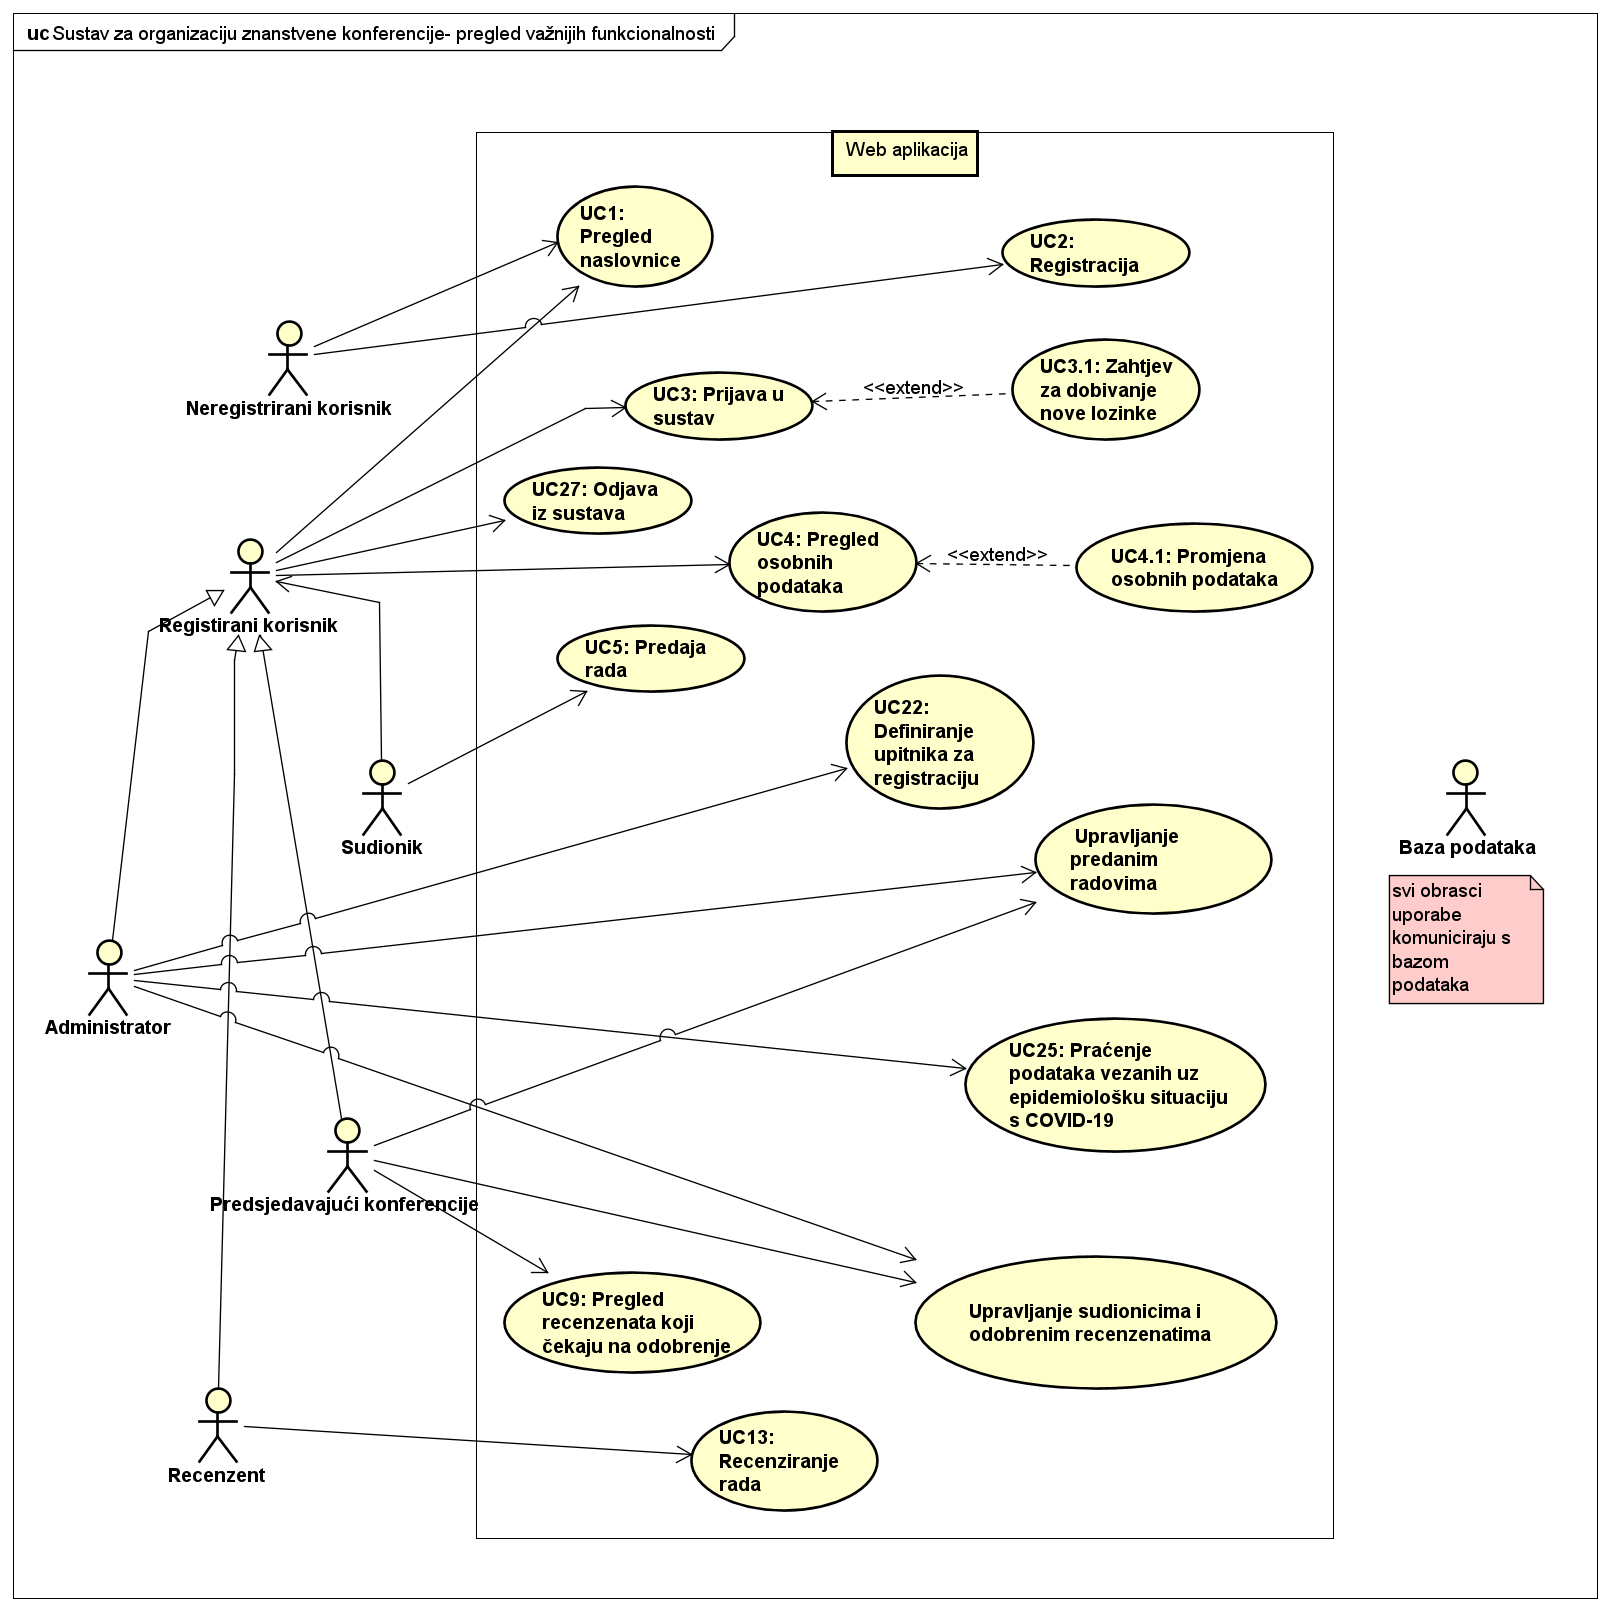
\includegraphics[scale=0.35]{dijagrami/pregledvaznijihfunkcionalnosti.png} 
						\centering
						\caption{Dijagram obrasca uporabe, pregled važnijih funkcionalnosti sustava}
						\label{fig:dijagramobrascauporabe1}
					\end{figure}
					\begin{figure}[H]
						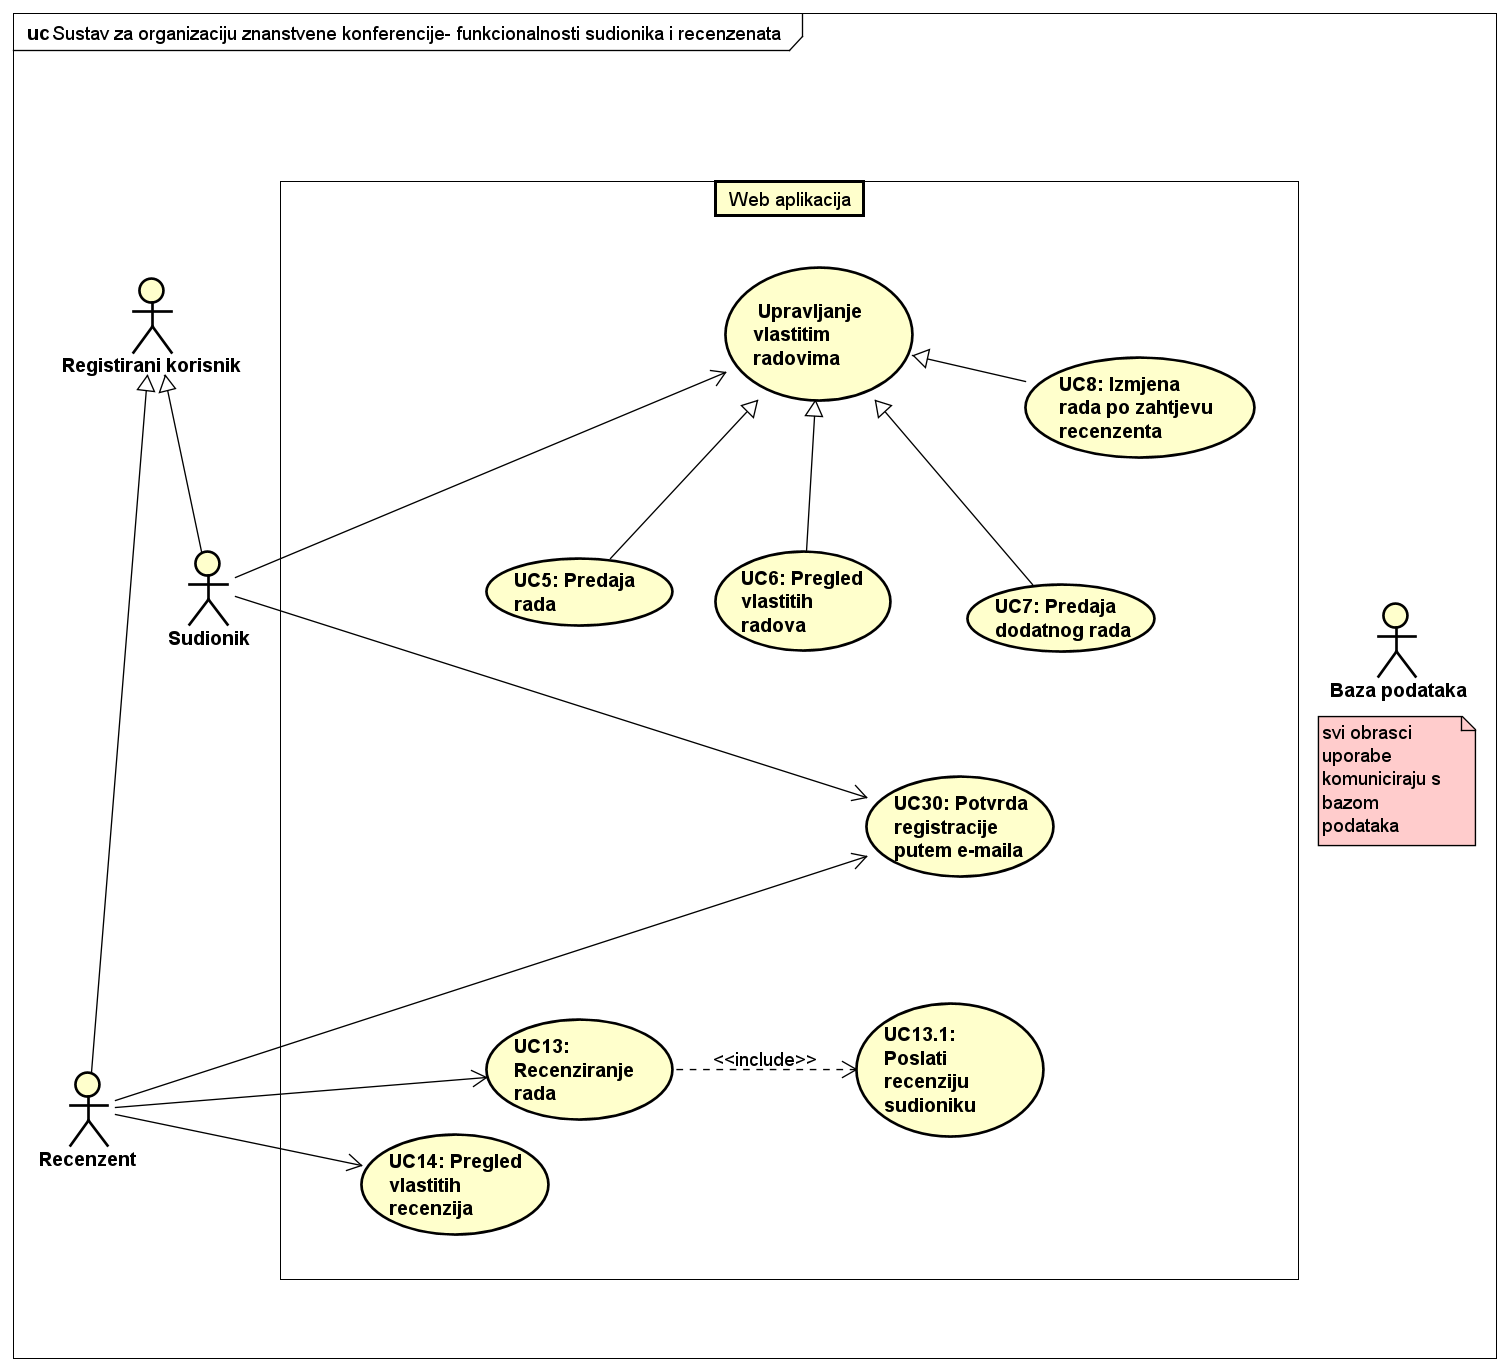
\includegraphics[scale=0.35]{dijagrami/funkcionalnosti-sudionici-recenzenti.png} 
						\centering
						\caption{Dijagram obrasca uporabe, funkcionalnosti sudionika i recenzenata}
						\label{fig:dijagramobrascauporabe2}
					\end{figure}
						\begin{figure}[H]
						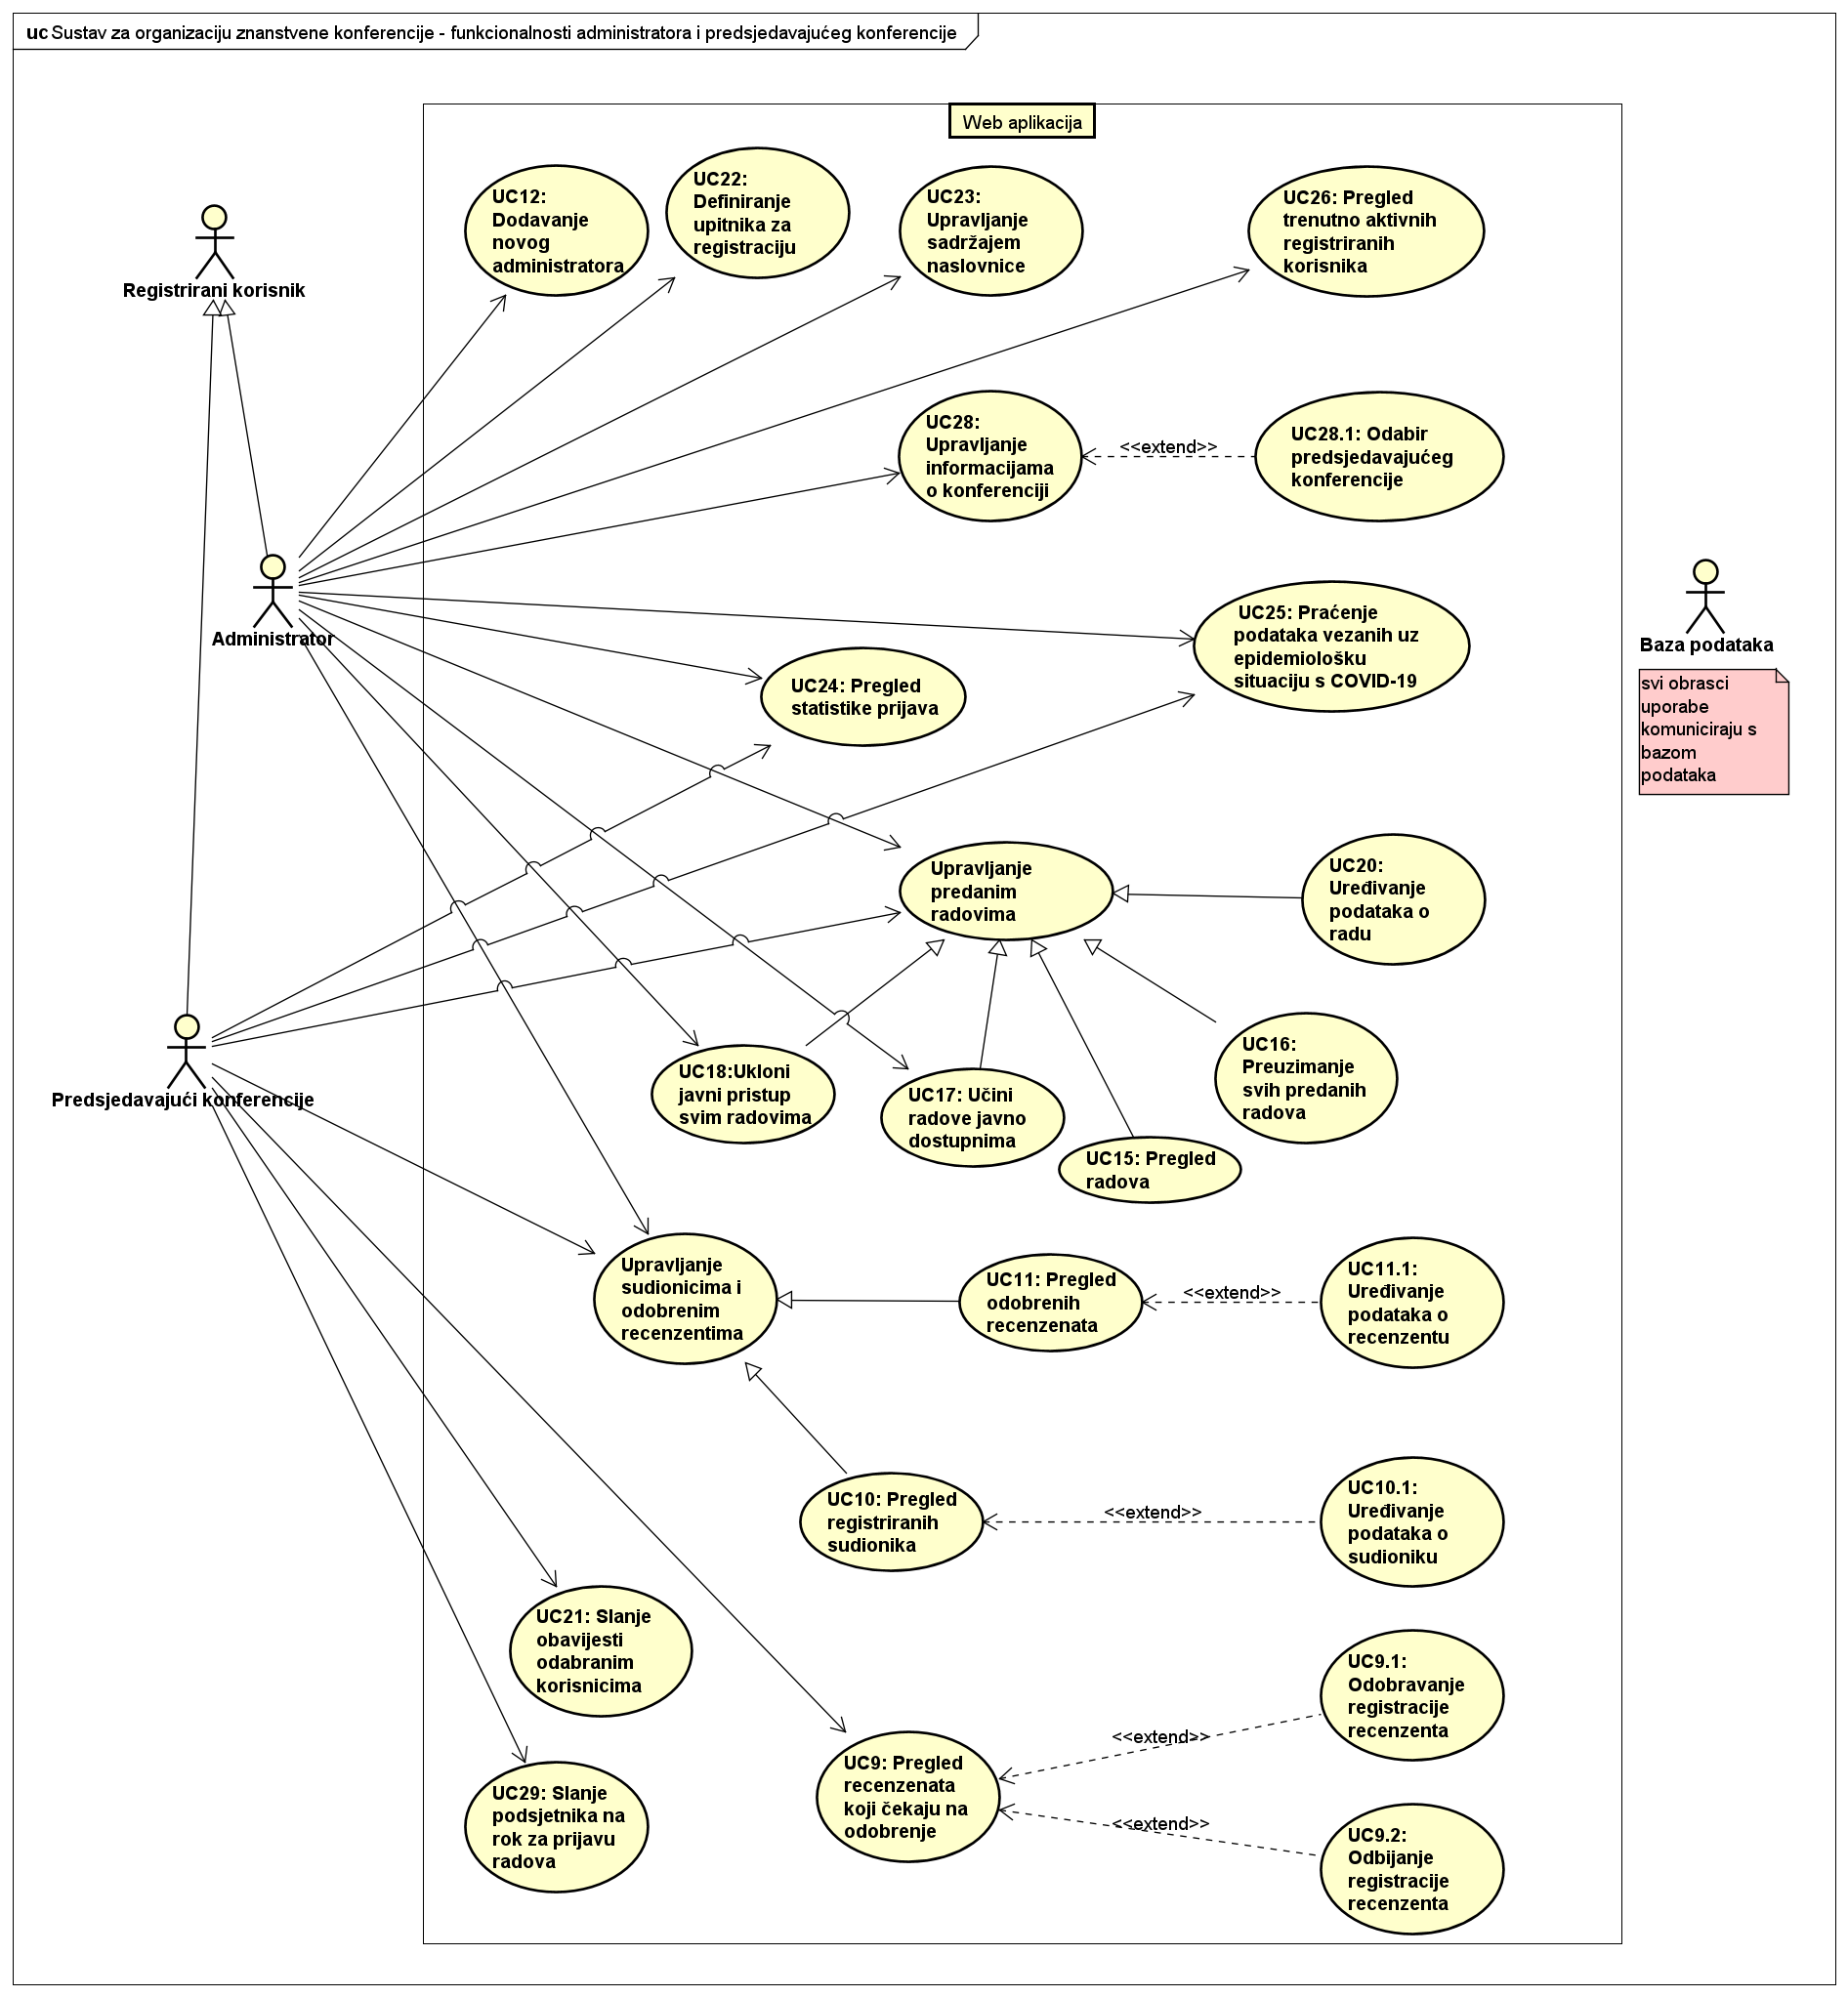
\includegraphics[height=16cm,width=15cm]{dijagrami/funkcionalnosti-administrator-predsjedavajucikonferencije.png} 
						\centering
						\caption{Dijagram obrasca uporabe, funkcionalnosti administratora i predsjedavajućeg konferencije}
						\label{fig:dijagramobrascauporabe3}
					\end{figure}
				\eject		
	
				
			\subsection{Sekvencijski dijagrami}
				
				\textbf{\textit{dio 1. revizije}}\\

				\textbf{Obrazac uporabe UC9 - Pregled recenzenata koji čekaju na odobrenje}\\
				Jedna od dužnosti predsjedavajućeg konferencije je odobriti registracije recenzenata. Kako bi odobrio ili odbio pojedinu registraciju, potrebno je otvoriti stranicu "Korisnici i radovi" te na njoj odabrati opciju "Popis recenzenata koji čekaju odobrenje". Ondje predsjedavajući može pregledavati registracije, odnosno podatke koje su pojedini recenzenti unijeli pri registraciji te na temelju toga odlučiti hoće li im odobriti ili odbiti prijavu. Ukoliko odluči odbiti prijavu, potrebno je navesti razlog zašto je prijava odbijena, te će se navedeni razlog poslati u "odbijenici" korisniku na e-mail klikom na gumb "Odbij prijavu", nakon čega registracija ujedno biva trajno izbrisana iz baze podataka. Ukoliko predsjedavajući odluči potvrditi registraciju, klikom na gumb "Potvrdi registraciju" podaci iz registracije se koriste za kreiranje novog korisnika, tj. recenzenta u bazi, a recenzentu se na e-mail šalje automatizirana poruka o prijavi registracije.
				\eject

				\begin{figure}[H]
					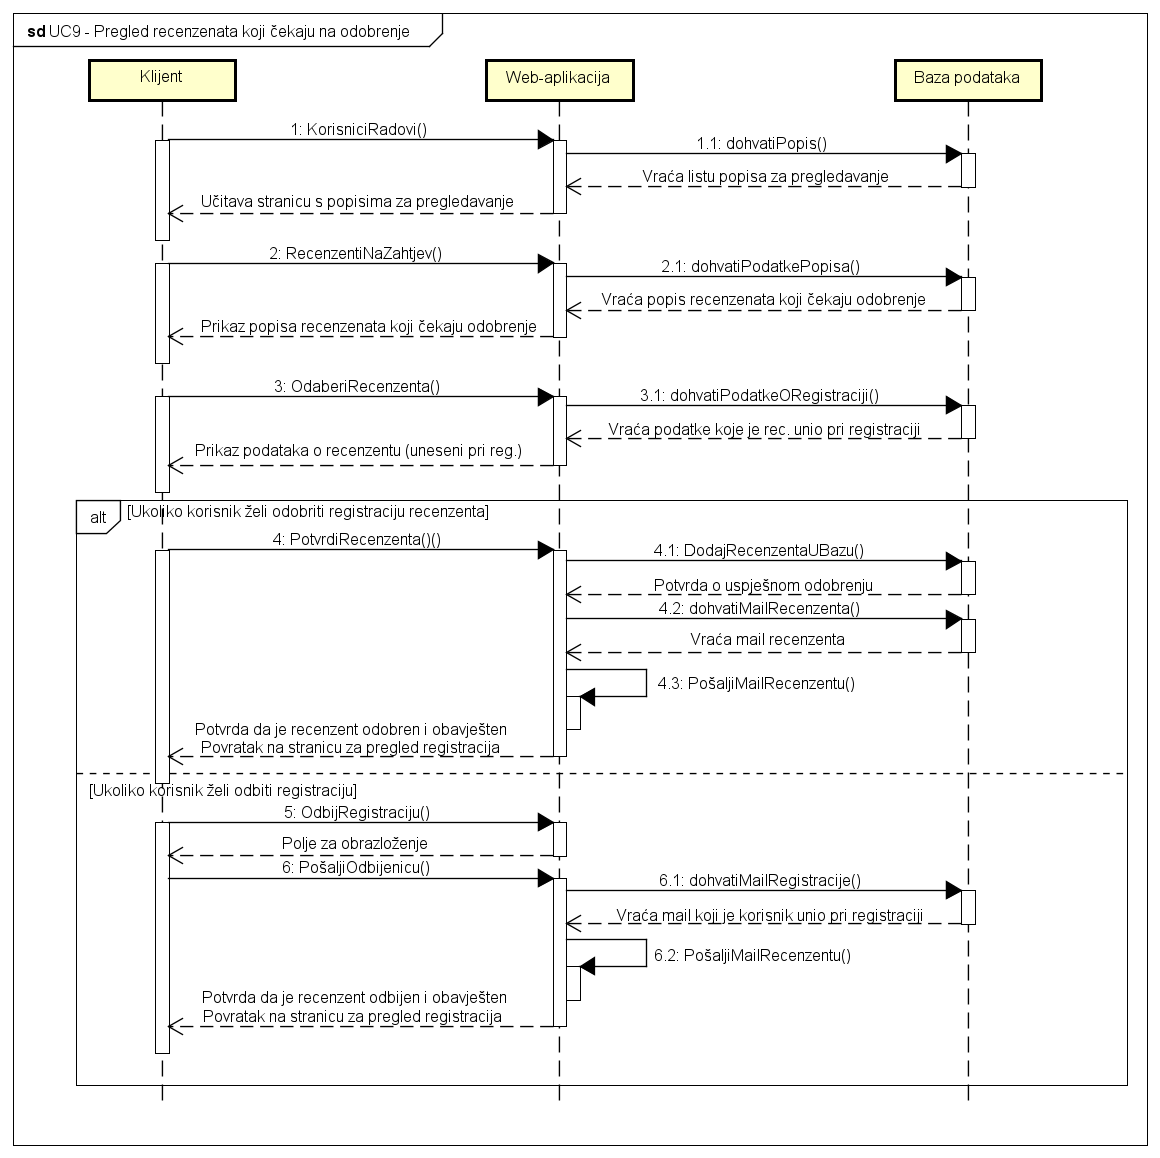
\includegraphics[scale=0.50]{dijagrami/UC9-RegistrRecenzent.png} 
					\centering
					\caption{Sekvencijski dijagram za UC9 - Pregled recenzenata koji čekaju na odobrenje}
					\label{fig:sekvencijski1}
				\end{figure}


				\eject
				
				\textbf{Obrazac uporabe UC13 - Recenziranje rada}\\
				Recenzent na stranici radova može koliko želi odabirati radove, čitati ih i pregledavati. Kada odabere i pročita rad koji namjerava recenzirati, a rad prethodno nije recenziran, kreće se prema dnu stranice gdje se nalazi odabir ocjene te mora odabrati jednu od četiri ocjene koje su definirane u opisu zadatka te je svakoj dodijeljen simboličan broj (u bazi podataka i u dokumentaciji). Bira jednu od 4 ocjene, te ovisno o tome koju ocjenu je odabrao (ukoliko su to ocjene 2., 3. ili 4.) pojavljuje se polje za upis obrazloženja ocjene. Korisnik može mijenjati ocjenu klikom sve dok se ne odluči za svoju konačnu ocjenu (i po potrebi unese obrazloženje ocjene), nakon čega korisnik bira opciju "Recenziraj ovaj rad". Klikom na navedenu opciju, recenzija se pohranjuje u bazi podataka (te je sukladno dostupna na stranici "Moje recenzije").
				\eject

				\begin{figure}[H]
					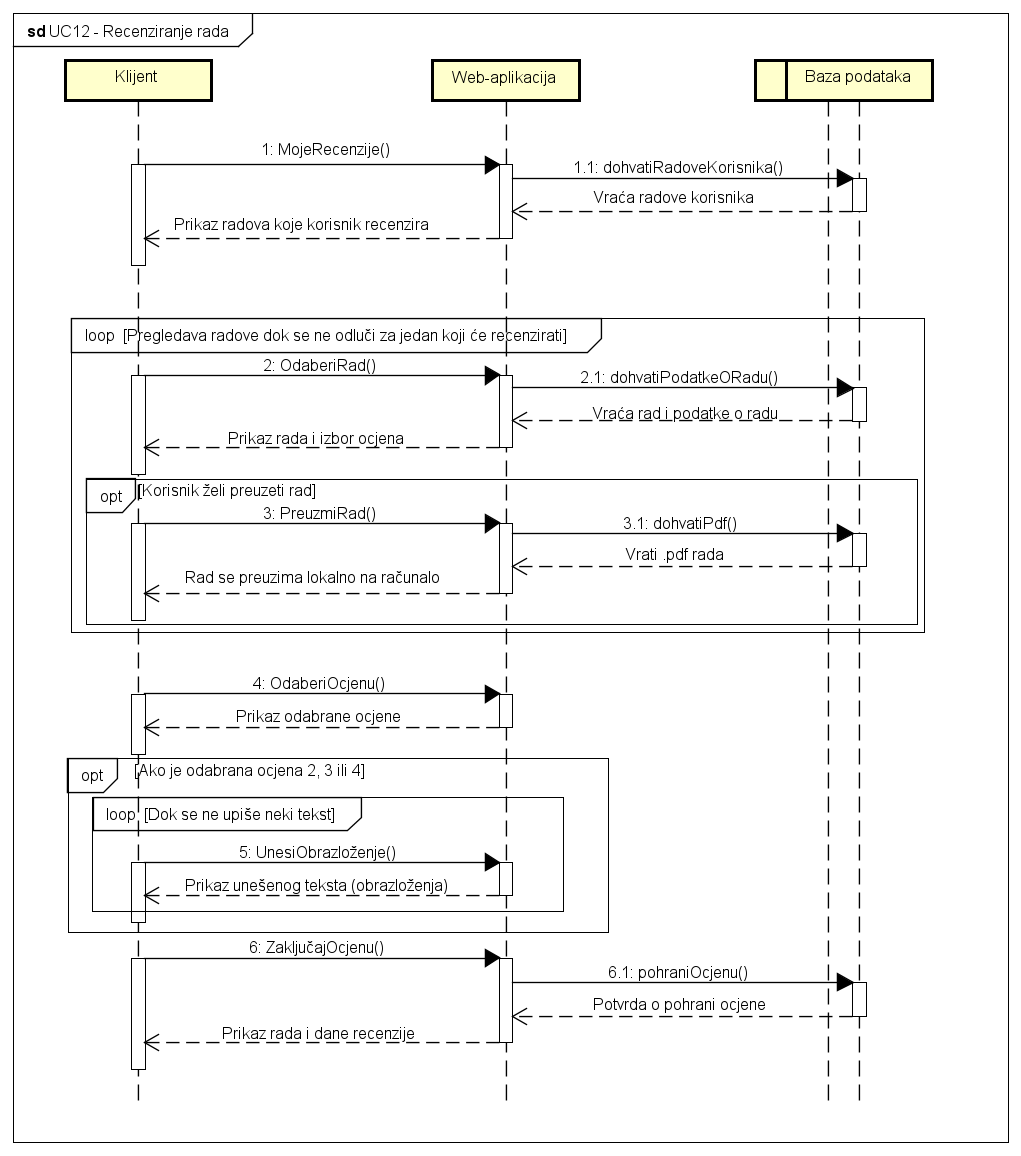
\includegraphics[scale=0.58]{dijagrami/UC13-RecenziranjeRada.png} 
					\centering
					\caption{Sekvencijski dijagram za UC13 - Recenziranje rada}
					\label{fig:sekvencijski2}
				\end{figure}


				\eject


				\textbf{Obrazac uporabe UC21 - Slanje obavijesti svim sudionicima i recenzentima}\\
				Administrator i predsjedavajući konferencije imaju mogućnost, ukoliko se ukaže potreba, poslati obavijest svim sudionicima i recenzentima (o bilokakvoj promjeni vezanoj za konferenciju i sl.). Isto čini tako da pristupi stranici "Administracijsko sučelje" te odabere opciju na vrhu stranice "Pošalji obavijest svima" pri čemu se otvara stranica s poljem za unos teksta obavijesti. Korisnik unosi tekst obavijesti, a kad je siguran da želi poslati obavijest bira opciju "Pošalji". Iz baze podataka dohvaćaju se e-mail adrese svih sudionika i recenzenata te se putem Web-aplikacije šalje e-mail na sve adrese povučene iz baze podataka. Korisnik prima obavijest o uspješnom slanju obavijesti.
				\eject

				\begin{figure}[H]
					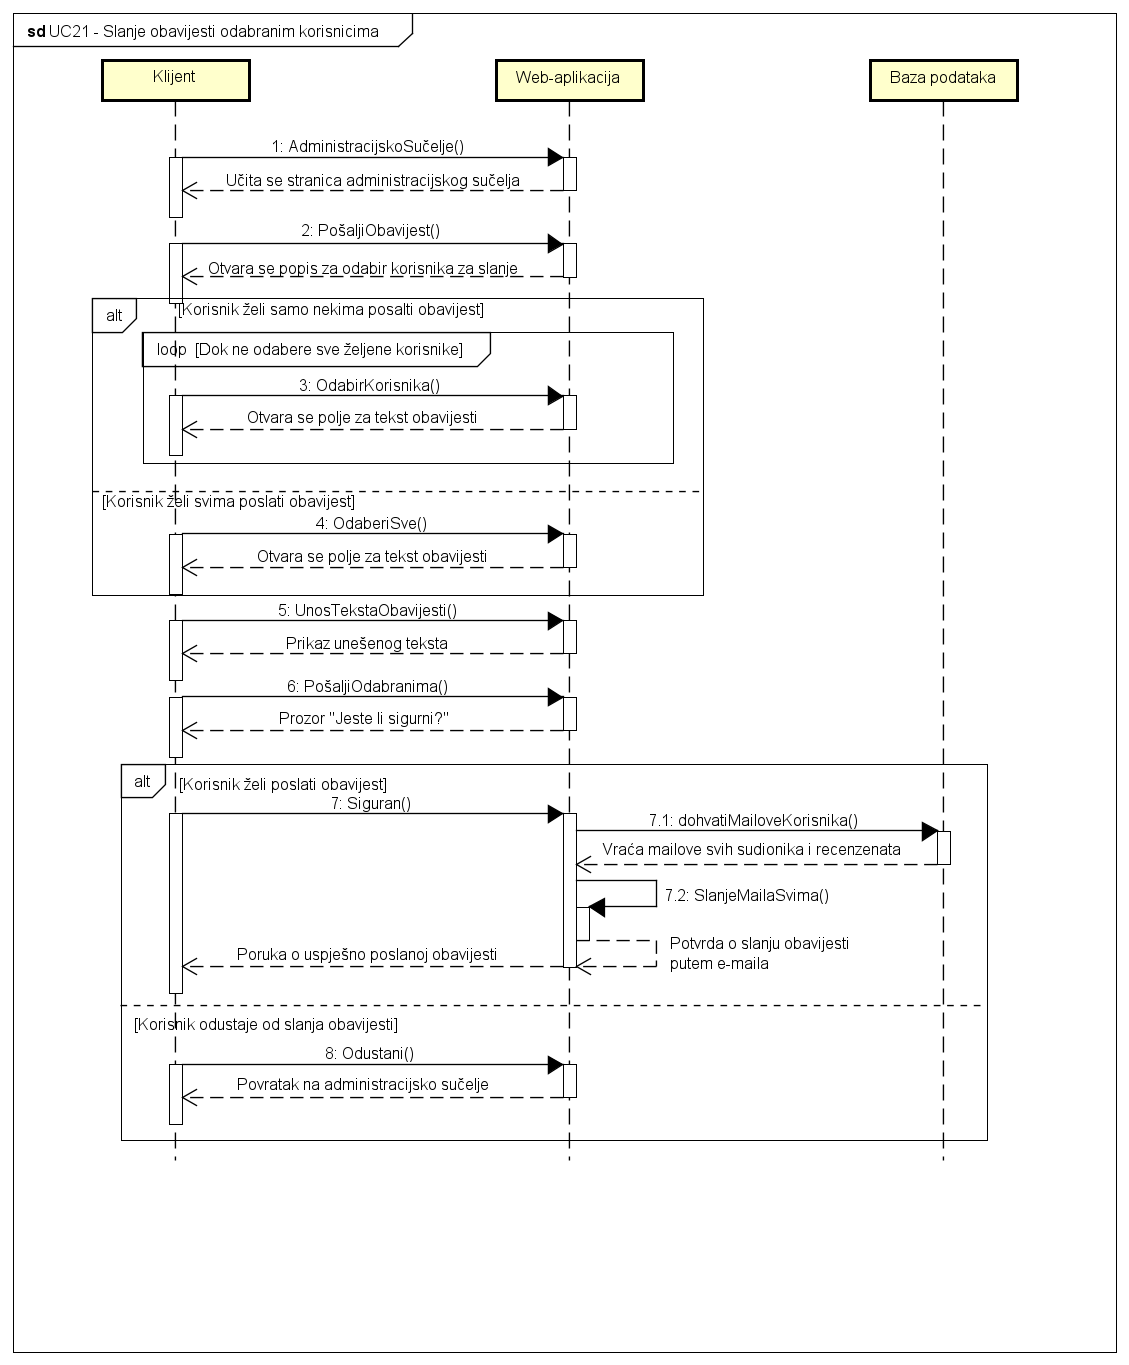
\includegraphics[scale=0.50]{dijagrami/UC21-SlanjeMaila.png} 
					\centering
					\caption{Sekvencijski dijagram za UC21 - Slanje obavijesti svim sudionicima i recenzentima}
					\label{fig:sekvencijski3}
				\end{figure}

				\eject

				\textbf{Obrazac uporabe UC28 - Upravljanje informacijama o konferenciji}\\
				Administrator je dužan ažurirati informacije o konferenciji, što čini preko stranice "informacije o konferenciji". Tamo može, između ostaloga, prvi puta odabrati predsjedavajućeg konferencije, a kasnije može i mijenjati podatke o njemu (promijeniti osobne podatke, unijeti novu e-mail adresu i sl.). Ukoliko administrator promijeni e-mail adresu predsjedavajućeg, na novu e-mail adresu dolazi poruka s lozinkom za prijavu u sustav. Nadalje, na navedenoj stranici može odabrati odsječak po svojoj želji, kliknuti gumb "Uredi", izmijeniti podatke te na kraju odabrati "Ažuriraj podatke". Pri tome se baza podataka ažurira, kao i stranica koju sudionici i recenzenti vide.
				\eject

				\begin{figure}[H]
					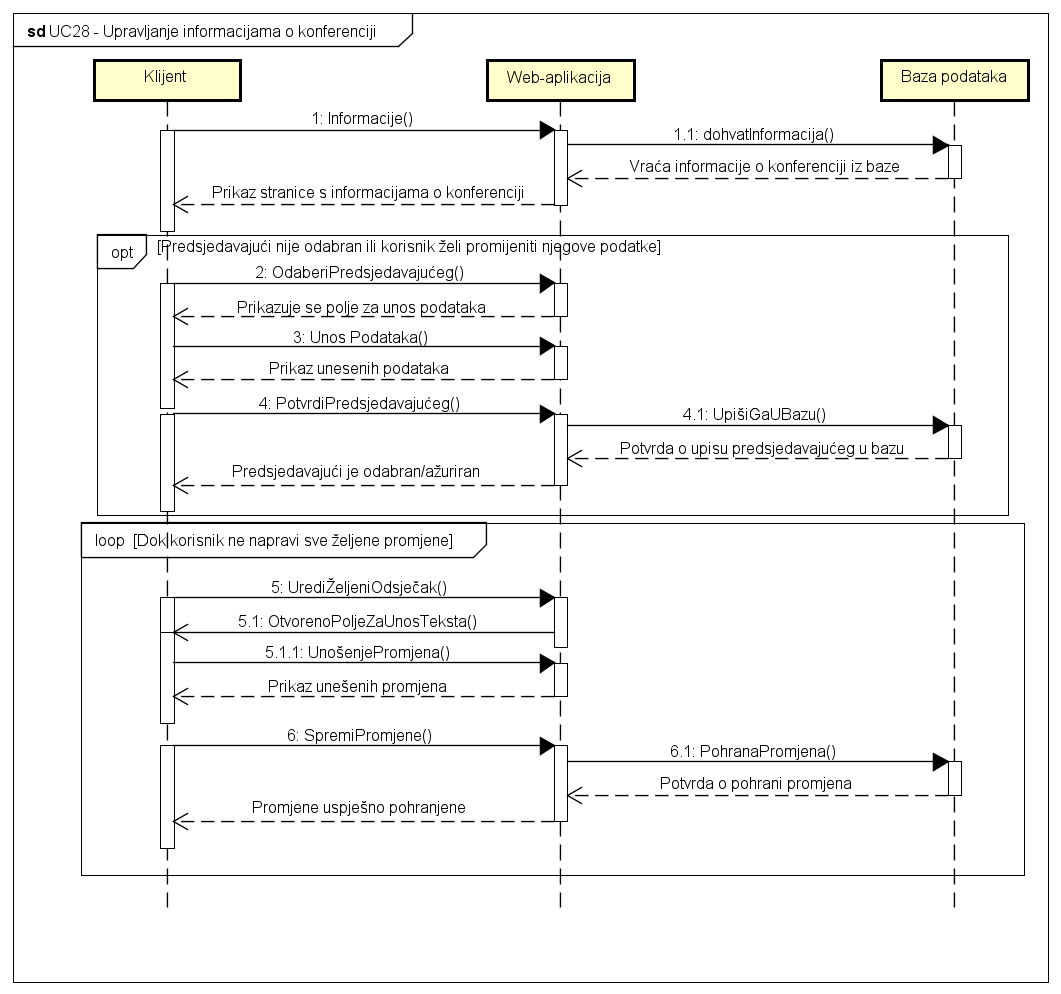
\includegraphics[scale=0.50]{dijagrami/UC28-UprInfoAdmin.png} 
					\centering
					\caption{Sekvencijski dijagram za UC28 - Upravljanje informacijama o konferenciji}
					\label{fig:sekvencijski4}
				\end{figure}

				\eject

	
		\section{Ostali zahtjevi}
		
			\textbf{\textit{dio 1. revizije}}\\
		 
			 \begin{packed_item}

				\item Sustav treba omogućiti istovremeni rad više korisnika, isto kao što i treba osigurati da svaki korisnik ima jedinstvenu i sigurnu zaporku s kojom se prijavljuju u sustav. Također, svi korisnici koji vrše registraciju daju privolu da pristaju na prikupljanje i daljnju obradu osobnih podataka sukladno sa zakonom o zaštiti podataka (GDPR). Sustav će koristiti protokol HTTPS za komunikaciju između korisnika i servera.
				\item Sustav treba spriječiti višestruku prijavu istog rada (radova istog naslova i autora).
				\item Sustav treba biti jednostavan i intuitivan za korištenje, a implementiran je kao web-aplikacija kreirana korištenjem objektno-orijentiranih jezika.
				\item Veza s bazom podataka mora biti zaštićena, brza i otporna na vanjske greške.
				\item Neispravno korištenje sučelja ne smije narušiti rad sustava. Korisničko sučelje i sustav moraju podržavati hrvatsku abecedu pri unosu tekstualnog sadržaja

			\end{packed_item}
			 
			 
			 
	